%! Author = wys
%! Date = 2020/9/23

% Preamble
\documentclass[a4paper, 12pt, AutoFakeBold, AutoFakeSlant]{article}

% Packages
\usepackage{xeCJK}
\usepackage{indentfirst}
\usepackage{listings}
\usepackage{enumitem}
\usepackage{graphicx}
\usepackage{amsmath}
\usepackage[colorlinks, linkcolor=black]{hyperref}
\usepackage{xcolor}
\usepackage[font={it}]{caption}
\usepackage[numbered]{bookmark}

\setCJKmainfont{宋体}
\setCJKmonofont{宋体}
\setmainfont{Times New Roman}
\setmonofont{Noto Sans Mono}
\linespread{1.25}
\CJKsetecglue{\,}
\numberwithin{figure}{section}

\lstset{
basicstyle = \ttfamily\footnotesize,
breakatwhitespace = false,
breaklines = true,
commentstyle = \color{gray}\itshape,
extendedchars = false,
keepspaces=true,
keywordstyle=\color{blue}, % keyword style
language = C++,            % the language of code
otherkeywords={string},
rulecolor=\color{black},
showspaces=false,
showstringspaces=false,
showtabs=false,
stringstyle=\color{magenta},        % string literal style
tabsize=4,
}

%\includeonly{ch7}

% Document
\begin{document}
    \tableofcontents
    \clearpage
    \setcounter{page}{1}


    \part{基本语言特性}\label{part1}
    这一部分介绍了C++17中新的核心语言特性,但不包括那些专为泛型编程(即template)设计的特性。
    这些新增的特性对于应用程序员的日常编程非常有用,因此每一个使用C++17的C++程序员都应该了解它们。

    专为模板编程设计的新的核心语言特性在\autoref{part2}中介绍。

    \section{结构化绑定}\label{ch1}
结构化绑定允许你用一个对象的元素或成员同时实例化多个实体。
例如,假设你定义了一个有两个不同成员的结构体:
\begin{lstlisting}
    struct MyStruct {
        int i = 0;
        std::string s;
    };

    MyStruct ms;
\end{lstlisting}
你可以通过如下的声明直接把该结构体的两个成员绑定到新的变量名:
\begin{lstlisting}
    auto [u, v] = ms;
\end{lstlisting}
这里,变量\texttt{u}和\texttt{v}的声明方式称为\emph{结构化绑定}。
某种程度上可以说它们解构了用来初始化的对象(在某些地方它们被称为\emph{解构声明})。

如下的每一种声明方式都是支持的:
\begin{lstlisting}
    auto [u2, v2] {ms};
    auto [u3, v3] (ms);
\end{lstlisting}
结构化绑定对于返回结构体或者数组的函数来说非常有用。例如,考虑一个返回结构体的函数:
\begin{lstlisting}
    MyStruct getStruct() {
        return MyStruct{42, "hello"};
    }
\end{lstlisting}
你可以直接把返回的数据成员赋值给两个新的局部变量:
\begin{lstlisting}
    auto [id, val] = getStruct();  // id和val分别是返回结构体的i和s成员
\end{lstlisting}
这个例子中,\texttt{id}和\texttt{val}分别是返回结构体中的\texttt{i}和\texttt{s}成员。
它们的类型分别是\texttt{int}和\texttt{std::string},可以被当作两个不同的对象来使用:
\begin{lstlisting}
    if (id > 30) {
        std::cout << val;
    }
\end{lstlisting}
这么做的好处是可以直接访问成员,
另外,把值绑定到能体现语义的变量名上,可以使代码的可读性更强。\footnote{感谢Zachary Turner指出这一点}

下面的代码演示了使用结构化绑定能带来怎样的显著改进。
在不使用结构化绑定的情况下遍历\texttt{std::map<>}的元素需要这么写:
\begin{lstlisting}
    for (const auto& elem : mymap) {
        std::cout << elem.first << ": " << elem.second << '\n';
    }
\end{lstlisting}
map的元素的类型是键和值组成的\texttt{std::pair}类型,
\texttt{std::pair}的成员分别是\texttt{first}和\texttt{second},
上边的例子中必须使用成员的名字来访问键和值。通过使用结构化绑定,代码的可读性大大提升:
\begin{lstlisting}
    for (const auto& [key, val] : mymap) {
        std::cout << key << ": " << val << '\n';
    }
\end{lstlisting}
上面的例子中我们可以使用准确体现语义的变量名直接访问每一个元素。

\subsection{细说结构化绑定}
为了理解结构化绑定,必须意识到这里面其实有一个隐藏的匿名对象。
结构化绑定时新引入的局部变量名其实都指向这个匿名对象的成员/元素。

\subsubsection*{绑定到一个匿名实体}
如下代码的精确行为:
\begin{lstlisting}
    auto [u, v] = ms;
\end{lstlisting}
等价于我们用\texttt{ms}初始化了一个新的实体\texttt{e},
并且让结构化绑定中的\texttt{u}和\texttt{v}变成了\texttt{e}的成员的别名,类似于如下定义:
\begin{lstlisting}
    auto e = ms;
    aliasname u = e.i;
    aliasname v = e.s;
\end{lstlisting}
这意味着\texttt{u}和\texttt{v}仅仅是\texttt{ms}的一份本地拷贝的成员的别名。
然而,我们没有为\texttt{e}声明一个名称,因此我们不能直接访问这个匿名对象。
注意\texttt{u}和\texttt{v}并不是\texttt{e.i}和\texttt{e.s}的引用(而是它们的别名)。
\texttt{decltype(u)}的结果是成员\texttt{i}的类型,
\texttt{declytpe(v)}的结果是成员\texttt{s}的类型。
因此:
\begin{lstlisting}
    std::cout << u << ' ' << v << '\n';
\end{lstlisting}
会打印出\texttt{e.i}和\texttt{e.s}(分别是\texttt{ms.i}和\texttt{ms.s}的拷贝)。

\texttt{e}的生命周期和结构化绑定的生命周期相同,当结构化绑定离开作用域时\texttt{e}也会被自动销毁。
另外,除非使用了引用,否则修改结构化绑定的变量并不会影响被绑定的变量:
\begin{lstlisting}
    MyStruct ms{42, "hello"};
    auto [u, v] = ms;
    ms.i = 77;
    std::cout << u;     // 打印出42
    u = 99;
    std::cout << ms.i;  // 打印出77
\end{lstlisting}
在这个例子中\texttt{u}和\texttt{ms.i}有不同的内存地址。

当使用结构化绑定来绑定返回值时,规则是相同的。如下初始化
\begin{lstlisting}
    auto [u, v] = getStruct();
\end{lstlisting}
的行为等价于我们用\texttt{getStruct()}的返回值初始化了一个新的实体\texttt{e},
之后结构化绑定的变量\texttt{u}和\texttt{v}变成了\texttt{e}的两个成员的别名,类似于如下定义:
\begin{lstlisting}
    auto e = getStruct();
    aliasname u = e.i;
    aliasname v = e.s;
\end{lstlisting}
也就是说,结构化绑定绑定到了一个新的实体\texttt{e}上,而不是直接绑定到了返回值上。
匿名实体\texttt{e}同样遵循通常的内存对齐规则,结构化绑定的每一个变量都会根据相应成员的类型进行对齐。

\subsubsection*{使用修饰符}
我们可以在结构化绑定中使用修饰符,例如\texttt{const}和引用,这些修饰符会作用在匿名实体\texttt{e}上。
通常情况下,作用在匿名实体上和作用在结构化绑定的变量上的效果是一样的,但有些时候又是不同的(见下文)。

例如,我们可以把声明一个结构化绑定声明为\texttt{const}引用:
\begin{lstlisting}
    const auto& [u, v] = ms;    // 引用,因此u/v指向ms.i/ms.s
\end{lstlisting}
这里,匿名实体被声明为\texttt{const}引用,
而\texttt{u}和\texttt{v}分别是这个引用的成员\texttt{i}和\texttt{s}的别名。
因此,对\texttt{ms}的成员的修改会影响到\texttt{u}和\texttt{v}的值:
\begin{lstlisting}
    ms.i = 77;          // 影响u的值
    std::cout << u;     // 打印出77
\end{lstlisting}
如果声明为非\texttt{const}引用,你甚至可以修改对象的成员:
\begin{lstlisting}
    MyStruct ms{42, "hello"};
    auto& [u, v] = ms;      // 被初始化的实体是ms的引用
    ms.i = 77;              // 影响到u的值
    std::cout << u;         // 打印出77
    u = 99;                 // 修改了ms.i
    std::cout << ms.i;      // 打印出99
\end{lstlisting}
如果一个结构化绑定是引用类型,而且是对一个临时对象的引用,那么和往常一样,
临时对象的生命周期会被延长到结构化绑定的生命周期:
\begin{lstlisting}
    MyStruct getStruct();
    ...
    const auto& [a, b] = getStruct();
    std::cout << "a: " << a << '\n';    // OK
\end{lstlisting}

\subsubsection*{修饰符并不是作用在结构化绑定引入的变量上}
修饰符会作用在新的匿名实体上,而不是结构化绑定引入的新的变量名上。事实上,如下代码中:
\begin{lstlisting}
    const auto& [u, v] = ms;    // 引用,因此u/v指向ms.i/ms.s
\end{lstlisting}
\texttt{u}和\texttt{v}都不是引用,只有匿名实体\texttt{e}是一个引用。
\texttt{u}和\texttt{v}分别是\texttt{ms}对应的成员的类型,
只不过变成了\texttt{const}的。
根据我们的推导,\texttt{decltype(u)}是\texttt{const int},
\texttt{decltype(v)}是\texttt{const std::string}。

当声明对齐时也是类似:
\begin{lstlisting}
    alignas(16) auto [u, v] = ms;   // 对齐匿名实体,而不是v
\end{lstlisting}
这里,我们对齐了匿名实体而不是\texttt{u}和\texttt{v}。
这意味着\texttt{u}作为第一个成员会按照16字节对齐,但\texttt{v}不会。

因此,即使使用了\texttt{auto}结构化绑定也不会发生类型退化(\emph{decay})
\footnote{术语\emph{decay}是指当参数按值传递时发生的类型转换,
例如原生数组会转换为指针,顶层修饰符例如\texttt{const}和引用会被忽略}。
例如,如果我们有一个原生数组组成的结构体:
\begin{lstlisting}
    struct S {
        const char x[6];
        const char y[3];
    };
\end{lstlisting}
那么如下声明之后:
\begin{lstlisting}
    S s1{};
    auto [a, b] = s1;    // a和b的类型是结构体成员的精确类型
\end{lstlisting}
这里\texttt{a}的类型仍然是\texttt{char[6]}。
再次强调,\texttt{auto}关键字应用在匿名实体上,这里匿名实体整体并不会发生类型退化。
这和用\texttt{auto}初始化新对象不同,如下代码中会发生类型退化:
\begin{lstlisting}
    auto a2 = a;    // a2的类型是a的退化类型
\end{lstlisting}

\subsubsection*{move语义}
move语义也遵循之前介绍的规则,如下声明:
\begin{lstlisting}
    MyStruct ms = { 42, "Jim" };
    auto&& [v, n] = std::move(ms);     // 匿名实体是ms的右值引用
\end{lstlisting}
这里\texttt{v}和\texttt{n}指向的匿名实体是\texttt{ms}的右值引用。
同时\texttt{ms}的值仍然保持不变:
\begin{lstlisting}
    std::cout << "ms.s: " << ms.s << '\n';  // 打印出"Jim"
\end{lstlisting}
然而,你可以对指向\texttt{ms.s}的\texttt{n}进行移动赋值:
\begin{lstlisting}
    std::string s = std::move(n);           // 把ms.s移动到s
    std::cout << "ms.s: " << ms.s << '\n';  // 打印出未定义的值
    std::cout << "n:    " << n << '\n';     // 打印出未定义的值
    std::cout << "s:    " << s << '\n';     // 打印出"Jim"
\end{lstlisting}
像通常一样,值被移动走的对象处于一个值未定义但却有效的状态。因此可以打印它们的值,
但不要对打印出的值有任何期望。\footnote{对于\texttt{string}来说,
值被移动走之后一般是处于空字符串的状态,但并不保证这一点}

上面的例子和直接用\texttt{ms}被移动走的值进行结构化绑定有些不同:
\begin{lstlisting}
    MyStruct ms = {42, "Jim" };
    auto [v, n] = std::move(ms);    // 新的匿名实体持有从ms处移动走的值
\end{lstlisting}
这里新的匿名实体是用\texttt{ms}被移动走的值来初始化的。因此,\texttt{ms}已经失去了值:
\begin{lstlisting}
    std::cout << "ms.s: " << ms.s << '\n';  // 打印出未定义的值
    std::cout << "n:    " << n << '\n';     // 打印出"Jim"
\end{lstlisting}
你可以继续用\texttt{n}进行移动赋值或者给\texttt{n}赋予新值,但已经不会再影响到\texttt{ms.s}了:
\begin{lstlisting}
    std::string s = std::move(n);   // 把n移动到s
    n = "Lara";
    std::cout << "ms.s: " << ms.s << '\n';  // 打印出未定义的值
    std::cout << "n:    " << n << '\n';     // 打印出"Lara"
    std::cout << "s:    " << s << '\n';     // 打印出"Jim"
\end{lstlisting}

\subsection{结构化绑定的适用场景}
原则上讲,结构化绑定适用于所有只有\texttt{public}数据成员的结构体、
C风格数组和类似元组(tuple-like)的对象:
\begin{itemize}[leftmargin=*]
    \item 对于所有非静态数据成员都是\texttt{public}的\textbf{结构体和类},
    你可以把每一个成员绑定到一个新的变量名上。
    \item 对于\textbf{原生数组},你可以把数组的每一个元素都绑定到新的变量名上。
    \item 对于任何类型,你可以使用\textbf{tuple-like API}来绑定新的名称,
    无论这套API是如何定义“元素”的。对于一个类型\emph{type}这套API需要如下的组件:
    \begin{itemize}[leftmargin=*]
        \item \texttt{std::tuple\_size<type>::value}要返回元素的数量。
        \item \texttt{std::tuple\_element<idx, type>::type}
        要返回第\texttt{idx}个元素的类型。
        \item 一个全局或成员函数\texttt{get<idx>()}要返回第\texttt{idx}个元素的值。
    \end{itemize}
    标准库类型\texttt{std::pair<>}、\texttt{std::tuple<>}、\texttt{std::array<>}
    就是提供了这些API的例子。
\end{itemize}
如果结构体和类提供了tuple-like API,那么将会使用这些API进行绑定,而不是直接绑定数据成员。

在任何情况下,结构化绑定中声明的变量名的数量都必须和元素或数据成员的数量相同。
你不能跳过某个元素,也不能重复使用变量名。然而,你可以使用非常短的名称例如\texttt{'\_'}
(有的程序员喜欢这个名字,有的讨厌它,但注意全局命名空间不允许使用它),
但这个名字在同一个作用域只能使用一次:
\begin{lstlisting}
    auto [_, val1] = getStruct();   // OK
    auto [_, val2] = getStruct();   // ERROR:变量名_已经被使用过
\end{lstlisting}
目前还不支持嵌套化的结构化绑定。

下一小节将详细讨论结构化绑定的使用。

\subsubsection{结构体和类}
上面几节里已经介绍了对只有\texttt{public}成员的结构体和类使用结构化绑定的方法,
一个典型的应用是直接对包含多个数据的返回值使用结构化绑定。然而有一些边缘情况需要注意。

注意要使用结构化绑定需要继承时遵循一定的规则。所有的非静态数据成员必须在同一个类中定义
(也就是说,这些成员要么是全部直接来自于最终的类,要么是全部来自同一个父类):
\begin{lstlisting}
    struct B {
        int a = 1;
        int b = 2;
    };

    struct D1 : B {
    };
    auto [x, y] = D1{};     // OK

    struct D2 : B {
        int c = 3;
    };
    auto [i, j, k] = D2{};  // 编译期ERROR
\end{lstlisting}
注意只有当\texttt{public}成员的顺序保证是固定的时候你才应该使用结构化绑定。
否则如果\texttt{B}中的\texttt{int a}和\texttt{int b}的顺序发生了变化,
\texttt{x}和\texttt{y}的值也会随之变化。为了保证固定的顺序,
C++17为一些标准库结构体(例如\texttt{insert\_return\_type})定义了成员顺序。

联合还不支持使用结构化绑定。

\subsubsection{原生数组}
下面的代码用C风格数组的两个元素初始化了\texttt{x}和\texttt{y}:
\begin{lstlisting}
    int arr[] = { 47, 11 };
    auto [x, y] = arr;  // x和y是arr中的int元素的拷贝
    auto [z] = arr;     // ERROR:元素的数量不匹配
\end{lstlisting}
注意这是C++中少数几种原生数组会按值拷贝的场景之一。

只有当数组的长度已知时才可以使用结构化绑定。
数组作为按值传入的参数时不能使用结构化绑定,因为数组会\emph{退化(decay)}为相应的指针类型。

注意C++允许通过引用来返回带有大小信息的数组,结构化绑定可以应用于返回这种数组的函数:
\begin{lstlisting}
    auto getArr() -> int(&)[2]; // getArr()返回一个原生int数组的引用
    ...
    auto [x, y] = getArr();     // x和y是返回的数组中的int元素的拷贝
\end{lstlisting}
你也可以对\texttt{std::array}使用结构化绑定,这是通过下一节要讲述的tuple-like API来实现的。

\subsubsection{\texttt{std::pair}, \texttt{std::tuple}和\texttt{std::array}}
结构化绑定的机制是可拓展的,你可以为任何类型添加对结构化绑定的支持。
标准库中就为\texttt{std::pair<>}、\texttt{std::tuple<>}、
\texttt{std::array<>}添加了支持。

\subsubsection*{\texttt{std::array}}
例如,下面的代码为\texttt{getArray()}返回的\texttt{std::array<>}中的四个元素绑定了
新的变量名\texttt{a},\texttt{b},\texttt{c},\texttt{d}:
\begin{lstlisting}
    std::array<int, 4> getArray();
    ...
    auto [a, b, c, d] = getArray(); // a,b,c,d是返回值的拷贝中的四个元素的别名
\end{lstlisting}
这里\texttt{a},\texttt{b},\texttt{c},\texttt{d}被绑定到\texttt{getArray()}返回的
\texttt{std::array}的元素上。

使用非临时变量的\texttt{non-const}引用进行绑定,还可以进行修改操作。例如:
\begin{lstlisting}
    std::array<int, 4> stdarr { 1, 2, 3, 4 };
    ...
    auto& [a, b, c, d] = stdarr;
    a += 10;    // OK:修改了stdarr[0]

    const auto& [e, f, g, h] = stdarr;
    e += 10;    // ERROR:引用指向常量对象

    auto&& [i, j, k, l] = stdarr;
    i += 10;    // OK:修改了stdarr[0]

    auto [m, n, o, p] = stdarr;
    m += 10;    // OK:但是修改的是stdarr[0]的拷贝
\end{lstlisting}
然而像往常一样,我们不能用临时对象(prvalue)初始化一个非 \texttt{const}引用:
\begin{lstlisting}
    auto& [a, b, c, d] = getArray();    // ERROR
\end{lstlisting}

\subsubsection*{\texttt{std::tuple}}
下面的代码将\texttt{a},\texttt{b},\texttt{c}初始化为\texttt{getTuple()}返回的
\texttt{std::tuple<>}的拷贝的三个元素的别名:
\begin{lstlisting}
    std::tuple<char, float, std::string> getTuple();
    ...
    auto [a, b, c] = getTuple();    // a,b,c的类型和值与返回的tuple中相应的成员相同
\end{lstlisting}
其中\texttt{a}的类型是\texttt{char},\texttt{b}的类型是\texttt{float},
\texttt{c}的类型是\texttt{std::string}。

\subsubsection*{\texttt{std::pair}}
作为另一个例子,考虑如下对关联/无序容器的\texttt{insert()}成员的返回值进行处理的代码:
\begin{lstlisting}
    std::map<std::string, int> coll;
    auto ret = coll.insert({"new", 42});
    if (!ret.second) {
        // 如果插入失败,使用ret.first处理错误
        ...
    }
\end{lstlisting}
通过使用结构化绑定,而不是使用\texttt{std::pair<>}的\texttt{first}和
\texttt{second}成员,代码的可读性大大增强:
\begin{lstlisting}
    auto [pos, ok] = coll.insert({"new", 42});
    if (!ok) {
        // 如果插入失败,用pos处理错误
        ...
    }
\end{lstlisting}
注意在这种场景中,C++17中提供了一种使用\hyperref[ch2]{带初始化的\texttt{if}语句}
来进行改进的方法。

\subsubsection*{为\texttt{pair}和\texttt{tuple}的结构化绑定赋予新值}
在声明了一个结构化绑定之后,你通常不能同时修改所有绑定的变量,
因为结构化绑定只能一起声明但不能一起使用。然而,如果被赋的值可以赋给一个\texttt{std::pair<>}或\texttt{std::tuple<>} ,你可以使用\texttt{std::tie()}
把值一起赋给所有变量。例如:
\begin{lstlisting}
    std::tuple<char, float, std::string> getTuple();
    ...
    auto [a, b, c] = getTuple();    // a,b,c的类型和值与返回的tuple相同
    ...
    std::tie(a, b, c) = getTuple(); // a,b,c的值变为新返回的tuple的值
\end{lstlisting}
这种方法可以被用来处理返回多个值的循环,例如\hyperref[ch24.1.2]{在循环中使用搜索器}:
\begin{lstlisting}
    std::boyer_moore_searcher bmsearch{sub.begin(), sub.end()};
    for (auto [beg, end] = bmsearch(text.begin(), text.end());
         beg != text.end();
         std::tie(beg, end) = bmsearch(end, text.end())) {
        ...
    }
\end{lstlisting}

\subsection{为结构化绑定提供Tuple-Like API}
你可以通过\emph{tuple-like API}为任何类型添加对结构化绑定的支持,
就像标准库中为\texttt{std::pair<>}、\texttt{std::tuple<>}、\texttt{std::array<>}做的一样:

\subsubsection*{支持只读结构化绑定}
下面的例子演示了怎么为一个类型\texttt{Customer}添加结构化绑定支持,
类的定义如下:
\begin{lstlisting}[frame=single, title=lang/customer1.hpp]
    #include <string>
    #include <utility>  // for std::move()

    class Customer {
      private:
        std::string first;
        std::string last;
        long val;
      public:
        Customer (std::string f, std::string l, long v)
            : first{std::move(f)}, last{std::move(l)}, val{v} {
        }
        std::string getFirst() const {
            return first;
        }
        std::string getLast() const {
            return last;
        }
        long getValue() const {
            return val;
        }
    };
\end{lstlisting}
我们可以用如下代码添加tuple-like API:
\begin{lstlisting}[frame=single, title=lang/structbind1.hpp]
    #include "customer1.hpp"
    #include <utility>  // for tuple-like API

    // 为类Customer提供tulpe-like API:
    template<>
    struct std::tuple_size<Customer> {
        static constexpr int value = 3; // 有三个属性
    };

    template<>
    struct std::tuple_element<2, Customer> {
        using type = long;  // 最后一个属性的类型是long
    };
    template<std::size_t Idx>
    struct std::tuple_element<Idx, Customer> {
        using type = std::string;   // 其他的属性都是string
    };

    // 定义特化的getter:
    template<std::size_t> auto get(const Customer& c);
    template<> auto get<0>(const Customer& c) { return c.getFirst(); }
    template<> auto get<1>(const Customer& c) { return c.getLast(); }
    template<> auto get<2>(const Customer& c) { return c.getValue(); }
\end{lstlisting}
这里,我们为顾客的三个属性定义了tuple-like API,并映射到三个getter:
\begin{itemize}[leftmargin=*]
    \item 顾客的名(first name)是\texttt{std::string}类型
    \item 顾客的姓(last name)是\texttt{std::string}类型
    \item 顾客的消费金额是\texttt{long}类型
\end{itemize}
属性的数量被定义为\texttt{std::tuple\_size}模板函数对类\texttt{Customer}的特化版本:
\begin{lstlisting}
    template<>
    struct std::tuple_size<Customer> {
        static constexpr int value = 3; // 我们有3个属性
    };
\end{lstlisting}
属性的类型被定义为\texttt{std::tuple\_element}的特化版本:
\begin{lstlisting}
    template<>
    struct std::tuple_element<2, Customer> {
        using type = long;  // 最后一个属性是long类型
    };
    template<std::size_t Idx>
    struct std::tuple_element<Idx, Customer> {
        using type = std::string;   // 其他的属性是string
    };
\end{lstlisting}
第三个属性是\texttt{long},被定义为\texttt{Idx}为2时的完全特化版本。
其他的属性类型都是\texttt{std::string},被定义为部分特化版本(优先级比全特化版本低)。
这里的类型就是结构化绑定时\texttt{decltype}返回的类型。

最后,在和类\texttt{Customer}同级的命名空间中定义了函数\texttt{get<>()}的
重载版本作为getter\footnote{C++17标准也允许把\texttt{get<>()}函数定义为成员函数,
但这可能只是一个疏忽,因此不应该这么用}:
\begin{lstlisting}
    template<std::size_t> auto get(const Customer& c);
    template<> auto get<0>(const Customer& c) { return c.getFirst(); }
    template<> auto get<1>(const Customer& c) { return c.getLast(); }
    template<> auto get<2>(const Customer& c) { return c.getValue(); }
\end{lstlisting}
在这种情况下,我们有一个主函数模板的声明和针对所有情况的全特化版本。

注意函数模板的全特化版本必须使用和声明时相同的类型(包括返回值类型都必须完全相同)。
这是因为我们只是提供特化版本的实现,而不是新的声明。下面的代码将不能通过编译:
\begin{lstlisting}
    template<std::size_t> auto get(const Customer& c);
    template<> std::string get<0>(const Customer& c) { return c.getFirst(); }
    template<> std::string get<1>(const Customer& c) { return c.getLast(); }
    template<> long get<2>(const Customer& c) { return c.getValue(); }
\end{lstlisting}
通过使用新的\hyperref[ch10]{编译期\texttt{if}语句特性},我们可以把\texttt{get<>()}函数的实现
\label{编译期if实现get<>}
合并到一个函数里:
\begin{lstlisting}
    template<std::size_t I> auto get(const Customer& c) {
        static_assert(I < 3);
        if constexpr (I == 0) {
            return c.getFirst();
        }
        else if constexpr (I == 1) {
            return c.getLast();
        }
        else {  // I == 2
            return c.getValue();
        }
    }
\end{lstlisting}
有了这个API,我们就可以为类型\texttt{Customer}使用结构化绑定:
\begin{lstlisting}[frame=single, title=lang/structbind1.cpp]
    #include "structbind1.hpp"
    #include <iostream>

    int main()
    {
        Customer c{"Tim", "Starr", 42};
        auto [f, l, v] = c;

        std::cout << "f/l/v:    " << f << ' '
                  << l << ' ' << v << '\n';

        // 修改结构化绑定的变量
        std::string s{std::move(f)};
        l = "Waters";
        v += 10;
        std::cout << "f/l/v:    " << f << ' ' << l << ' ' << v << '\n';
        std::cout << "c:        " << c.getFirst() << ' '
                  << c.getLast() << ' ' << c.getValue() << '\n';
        std::cout << "s:        " << s << '\n';
    }
\end{lstlisting}
如下初始化之后:
\begin{lstlisting}
    auto [f, l, v] = c;
\end{lstlisting}
像之前的例子一样,\texttt{Customer c}被拷贝到一个匿名实体。
当结构化绑定离开作用域时匿名实体也被销毁。

另外,对于每一个绑定\texttt{f}、\texttt{l}、\texttt{v},
它们对应的\texttt{get<>()}函数都会被调用。
因为定义的\texttt{get<>}函数返回类型是\texttt{auto},所以这3个getter会返回成员的拷贝,
这意味着结构化绑定的变量的地址不同于\texttt{c}中成员的地址。
因此,修改\texttt{c}的值并不会影响绑定变量(反之亦然)。

使用结构化绑定等同于使用\texttt{get<>()}函数的返回值,因此:
\begin{lstlisting}
    std::cout << "f/l/v:    " << f << ' ' << l << ' ' << v << '\n';
\end{lstlisting}
只是简单的输出变量的值(并不会再次调用getter函数)。另外
\begin{lstlisting}
    std::string s{std::move(f)};
    l = "Waters";
    v += 10;
    std::cout << "f/l/v:    " << f << ' ' << l << ' ' << v << '\n';
\end{lstlisting}
这段代码修改了绑定变量的值。因此,这段程序总是有如下输出:
\begin{lstlisting}
    f/l/v:    Tim Starr 42
    f/l/v:     Waters 52
    c:        Tim Starr 42
    s:        Tim
\end{lstlisting}
第二行的输出依赖于被move的\texttt{string}的值,一般情况下是空值,但也有可能是其他有效的值。

你也可以在迭代一个元素类型是\texttt{Customer}的\texttt{vector}时使用结构化绑定:
\begin{lstlisting}
    std::vector<Customer> coll;
    ...
    for (const auto& [first, last, val] : coll) {
        std::cout << first << ' ' << last << ": " << val << '\n';
    }
\end{lstlisting}
在这个循环中,因为使用了\texttt{const auto\&}所以不会有\texttt{Customer}被拷贝。
然而,结构化绑定时会调用\texttt{get<>()}函数返回姓和名的拷贝。
之后,循环体内的输出语句中再次使用了结构化绑定,不需要再次调用getter。
最后在每一次迭代结束的时候,拷贝的\texttt{string}会被销毁。

注意对绑定变量使用\texttt{decltype}会推导出变量自身的类型,
不会受到匿名实体的类型修饰符的影响。也就是说这里\texttt{decltype(first)}的类型是
\texttt{const std::string}而不是引用。

\subsubsection*{支持可写结构化绑定}
实现tuple-like API时可以时候用返回\texttt{non-const}引用。这样结构化绑定就变得可写。
设想类\texttt{Customer}提供了读写成员的API\footnote{这个类的设计比较失败,
因为通过成员函数可以直接访问私有成员。然而用来演示怎么支持可写结构化绑定已经足够了}:
\begin{lstlisting}[frame=single, title=lang/customer2.hpp]
    #include <string>
    #include <utility>  // for std::move()

    class Customer {
      private:
        std::string first;
        std::string last;
        long val;
      public:
        Customer (std::string f, std::string l, long v)
            : first{std::move(f))}, last{std::move(l)}, val{v} {
        }
        const std::string& firstname() const {
            return first;
        }
        std::string& firstname() {
            return first;
        }
        const std::string& lastname() const {
            return last;
        }
        long value() const {
            return val;
        }
        long& value() {
            return val;
        }
    };
\end{lstlisting}

为了支持读写,我们需要为常量和非常量引用定义重载的getter:
\begin{lstlisting}[frame=single, title=lang/structbind2.hpp]
    #include "customer2.hpp"
    #include <utility>  // for tuple-like API

    // 为类Customer提供tuple-like API
    template<>
    struct std::tuple_size<Customer> {
        static constexpr int value = 3; // 有3个属性
    };

    template<>
    struct std::tuple_element<2, Customer> {
        using type = long;  // 最后一个属性是long类型
    }
    template<std::size_t Idx>
    struct std::tuple_element<Idx, Customer> {
        using type = std::string;   // 其他的属性是string
    }

    // 定义特化的getter:
    template<std::size_t I> decltype(auto) get(Customer& c) {
        static_assert(I < 3);
        if constexpr (I == 0) {
            return c.firstname();
        }
        else if constexpr (I == 1) {
            return c.lastname();
        }
        else {  // I == 2
            return c.value();
        }
    }
    template<std::size_t I> decltype(auto) get(const Customer& c) {
        static_assert(I < 3);
        if constexpr (I == 0) {
            return c.firstname();
        }
        else if constexpr (I == 1) {
            return c.lastname();
        }
        else {  // I == 2
            return c.value();
        }
    }
    template<std::size_t I> decltype(auto) get(Customer&& c) {
        static_assert(I < 3);
        if constexpr (I == 0) {
            return std::move(c.firstname());
        }
        else if constexpr (I == 1) {
            return std::move(c.lastname());
        }
        else {  // I == 2
            return c.value();
        }
    }
\end{lstlisting}
注意你必须提供这3个版本的特化来分别处理常量对象、非常量对象、可移动对象,
\footnote{标准库中还为\texttt{const\&\&}实现了第4个版本的\texttt{get<>()}
这么做是有原因的(见\url{https://wg21.link/lwg2485)}),
但如果只是想支持结构化绑定则不是必须的。}。
为了实现返回引用,你应该使用\texttt{decltype(auto)}
\footnote{\texttt{decltype(auto)}在C++14中引入,
它可以根据表达式的值类别(\emph{value category})来推导(返回)类型。
简单来说,将它设置为返回值类型之后引用会以引用返回,但临时值会以值返回。}。

这里我们又一次使用了\hyperref[ch10]{编译期\texttt{if}语句特性},
这可以让我们的getter的实现变得更加简单。如果没有这个特性,我们必须写出所有的全特化版本,例如:
\begin{lstlisting}
    template<std::size_t> decltype(auto) get(const Customer& c);
    template<std::size_t> decltype(auto) get(Customer& c);
    template<std::size_t> decltype(auto) get(Customer&& c);
    template<> decltype(auto) get<0>(const Customer& c) { return c.firstname(); }
    template<> decltype(auto) get<0>(Customer& c) { return c.firstname(); }
    template<> decltype(auto) get<0>(Customer&& c) { return c.firstname(); }
    template<> decltype(auto) get<1>(const Customer& c) { return c.lastname(); }
    template<> decltype(auto) get<1>(Customer& c) { return c.lastname(); }
    ...
\end{lstlisting}
再次强调,主函数模板声明必须和全特化版本拥有完全相同的签名(包括返回值)。
下面的代码不能通过编译:
\begin{lstlisting}
    template<std::size_t> decltype(auto) get(Customer& c);
    template<> std::string& get<0>(Customer& c) { return c.firstname(); }
    template<> std::string& get<1>(Customer& c) { return c.lastname(); }
    template<> long& get<2>(Customer& c) { return c.value(); }
\end{lstlisting}
你现在可以对\texttt{Customer}类使用结构化绑定了,并且还能通过绑定修改成员的值:
\begin{lstlisting}[frame=single, title=lang/structbind2.cpp]
    #include "structbind2.hpp"
    #include <iostream>

    int main()
    {
        Customer c{"Tim", "Starr", 42};
        auto [f, l, v] = c;
        std::cout << "f/l/v:    " << f << ' ' << l << ' ' << v << '\n';

        // 通过引用修改结构化绑定
        auto&& [f2, l2, v2] = c;
        std::string s{std::move(f2)};
        f2 = "Ringo";
        v2 += 10;
        std::cout << "f2/l2/v2: " << f2 << ' '
                  << l2 << ' ' << v2 << '\n';
        std::cout << "c:        " << c.firstname() << ' '
                  << c.lastname() << ' ' << c.value() << '\n';
        std::cout << "s:        " << s << '\n';
    }
\end{lstlisting}
程序的输出如下:
\begin{lstlisting}
    f/l/v:    Tim Starr 42
    f2/l2/v2: Ringo Starr 52
    c:        Ringo Starr 52
    s:        Tim
\end{lstlisting}

\subsection{后记}
结构化绑定最早由Herb Sutter、Bjarne Stroustrup、Gabriel Dos Reis在
\url{https://wg21.link/p0144r0}提出,当时提议使用花括号而不是方括号。
最终被接受的提案由Jens Maurer发表于\url{https://wg21.link/p0217r3}。

    \section{带初始化的\texttt{if}和\texttt{switch}语句}\label{ch2}
\texttt{if}和\texttt{switch}语句现在允许在条件表达式里添加一条初始化语句。
例如,你可以写:
\begin{lstlisting}
    if (status s = check(); s != status::success) {
        return s;
    }
\end{lstlisting}
这里初始化语句:
\begin{lstlisting}
    status s = check();
\end{lstlisting}
初始化了\texttt{s},\texttt{s}将在整个\texttt{if}语句中有效(包括\texttt{else}分支里)。

\subsection{带初始化的\texttt{if}语句}
在\texttt{if}语句的条件表达式里定义的变量将在整个\texttt{if}语句中生效,
包括\emph{then}和\emph{else}部分。例如:
\begin{lstlisting}
    if (std::ofstream strm = getLogStrm(); coll.empty()) {
        strm << "<no data>\n";
    }
    else {
        for (const auto& elem : coll) {
            strm << elem << '\n';
        }
    }
    // strm不再有效
\end{lstlisting}
在整个\texttt{if}语句结束时\texttt{strm}的析构函数会被调用。
另一个例子是关于锁的使用,假设我们要在并发的环境中执行一个依赖某些条件的任务:
\begin{lstlisting}
    if (std::lock_guard<std::mutex> lg{collMutex}; !coll.empty()) {
        std::cout << coll.front() << '\n';
    }
\end{lstlisting}
这个例子中,如果使用\nameref{ch9},可以改写成如下代码:
\begin{lstlisting}
    if (std::lock_guard lg{collMutex}; !coll.empty()) {
        std::cout << coll.front() << '\n';
    }
\end{lstlisting}
上面的代码等价于:
\begin{lstlisting}
    {
        std::lock_guard<std::mutex> lg{collMutex};
        if (!coll.empty()) {
            std::cout << coll.front() << '\n';
        }
    }
\end{lstlisting}
细微的区别在于前者中\texttt{lg}在\texttt{if}语句的作用域之内定义,
和条件语句在相同的作用域。

注意这个特性的效果和传统\texttt{for}循环里的初始化语句完全相同。
上面的例子中为了让\texttt{lock\_guard}生效,必须在初始化语句里明确声明一个变量名,
否则它就是一个临时变量,会在创建之后就立即销毁。因此,初始化一个没有变量名的临时
\texttt{lock\_guard}是一个逻辑错误,因为当执行到条件语句时锁就已经被释放了:
\begin{lstlisting}
    if (std::lock_guard<std::mutex>{collMutex};     // 运行时ERROR
        !coll.empty()) {                    // 锁已经被释放了
        std::cout << coll.front() << '\n';  // 锁已经被释放了
    }
\end{lstlisting}
原则上讲,使用简单的\texttt{\_}作为变量名就已经足够了:
\begin{lstlisting}
    if (std::lock_guard<std::mutex> _{collMutex};   // OK,但是...
        !coll.empty()) {
        std::cout << coll.front() << '\n';
    }
\end{lstlisting}
你也可以同时声明多个变量,并且可以在声明时初始化:
\begin{lstlisting}
    if (auto x = qqq1(), y = qqq2(); x != y) {
        std::cout << "return values " << x << " and " << y << "differ\n";
    }
\end{lstlisting}
或者:
\begin{lstlisting}
    if (auto x{qqq1()}, y{qqq2()}; x != y) {
        std::cout << "return values " << x << " and " << y << "differ\n";
    }
\end{lstlisting}
作为另一个例子,考虑向\texttt{map}或者\texttt{unordered map}插入元素。
你可以像下面这样检查是否成功:
\begin{lstlisting}
    std::map<std::string, int> coll;
    ...
    if (auto [pos, ok] = coll.insert({"new", 42}); !ok) {
        // 如果插入失败,用pos处理错误
        const auto& [key, val] = *pos;
        std::cout << "already there: " << key << '\n';
    }
\end{lstlisting}
这里,我们用了\nameref{ch1}来给返回的\texttt{pos}指向的值声明了新的名称,
而不是使用\texttt{first}和\texttt{second}成员。在C++17之前,相应的处理代码必须像下面这样写:
\begin{lstlisting}
    auto ret = coll.insert({"new", 42});
    if (!ret.second) {
        // 如果插入失败,用ret.first处理错误
        const auto& elem = *(ret.first);
        std::cout << "already there: " << elem.first << '\n';
    }
\end{lstlisting}
注意这个拓展也适用于\nameref{ch10}特性。

\subsection{带初始化的\texttt{switch}语句}
通过使用带初始化的\texttt{switch}语句,我们可以在控制流之前初始化一个对象/实体。
例如,我们可以先声明一个\nameref{ch20.2.3},然后再根据它的类别进行处理:
\begin{lstlisting}
    namespace fs = std::filesystem;
    ...
    switch (fs::path p{name}; status(p).type()) {
        case fs::file_type::not_found:
            std::cout << p << " not found\n";
            break;
        case fs::file_type::directory:
            std::cout << p << ":\n";
            for (const auto& e : std::filesystem::directory_iterator{p}) {
                std::cout << "- " << e.path() << '\n';
            }
            break;
        default:
            std::cout << p << " exists\n";
            break;
    }
\end{lstlisting}
这里,初始化的路径\texttt{p}可以在整个\texttt{switch}语句中使用。

\subsection{后记}
带初始化语句的\texttt{if}和\texttt{switch}语句最早由Thomas Köppe
在\url{https://wg21.link/p0305r0}中提出,一开始只是提到了扩展\texttt{if}语句。
最终被接受的正式提案由Thomas Köpped发表于\url{https://wg21.link/p0305r1}。
    \section{内联变量}\label{ch3}
出于可移植性和易于整合的目的,提供包含类库声明的头文件是很重要的。
然而,在C++17之前,只有当这个库既不提供也不需要全局对象的时候才可以直接在头文件定义。

自从C++17开始,你可以在头文件中以\texttt{inline}的方式\emph{定义}全局变量/对象:
\begin{lstlisting}
    class MyClass {
        inline static std::string msg{"OK"}:    // 自从C++17起OK
        ...
    };

    inline MyClass myGlobalObj  // 即使被多个CPP文件包含也OK
\end{lstlisting}
只要一个翻译单元内没有重复的定义即可。此例中的定义即使被多个翻译单元使用,
也会指向同一个对象。

\subsection{内联变量产生的动机}
在C++里不允许在类里初始化非常量静态成员:
\begin{lstlisting}
    class MyClass {
        static std::string msg{"OK"};   // 编译期ERROR
        ...
    };
\end{lstlisting}
可以在类定义的外部定义并初始化非常量静态成员,但如果被多个CPP文件同时包含的话又会引发新的错误:
\begin{lstlisting}
    class MyClass {
        static std::string msg;
        ...
    };
    std::string MyClass::msg{"OK"}; // 如果被多个CPP文件包含会导致链接ERROR
\end{lstlisting}
根据\emph{一次定义原则}(ODR),一个变量或实体的定义只能出现在一个翻译单元内——
除非该变量或实体被定义为\texttt{inline}的。

即使使用预处理来进行保护也没有用:
\begin{lstlisting}
    #ifndef MYHEADER_HPP
    #define MYHEADER_HPP

    class MyClass {
        static std::string msg;
        ...
    };
    std::string MyClass::msg{"OK"}; // 如果被多个CPP文件包含会导致链接ERROR

    #endif
\end{lstlisting}
问题不在于头文件可能被重复包含多次,问题在于两个不同的CPP文件都包含了这个头文件,
因此都定义了\texttt{MyClass::msg}。出于同样的原因,如果你在头文件中定义了一个类的实例对象
也会出现相同的链接错误:
\begin{lstlisting}
    class MyClass {
        ...
    };
    MyClass myGlobalObject; // 如果被多个CPP文件包含会导致链接ERROR
\end{lstlisting}

\subsubsection*{解决方法}
对于一些场景,这里有一些解决方法:
\begin{itemize}[leftmargin=*]
    \item 你可以在一个\texttt{class/struct}的定义中初始化数字或枚举类型的常量静态成员:
    \begin{lstlisting}
    class MyClass {
        static const bool trace = false;    // OK,字面类型
        ...
    };
    \end{lstlisting}
    然而,这种方法只能初始化字面类型,例如基本的整数、浮点数、指针类型或者
    用常量表达式初始化了所有内部非静态成员的类,并且该类不能有用户自定义的或虚的析构函数。
    另外,如果你需要获取这个静态常量成员的地址(例如你想定义一个指向它的引用)的话
    那么你必须在那个翻译单元内定义它并且不能在其他翻译单元内再次定义。
    \item 你可以定义一个返回\texttt{static}的局部变量的内联函数:
    \begin{lstlisting}
    inline std::string& getMsg() {
        static std::string msg{"OK"};
        return msg;
    }
    \end{lstlisting}
    \item 你可以定义一个返回该值的\texttt{static}的成员函数:
    \begin{lstlisting}
    class MyClass {
        static std::string& getMsg() {
            static std::string msg{"OK"};
            return msg;
        }
        ...
    };
    \end{lstlisting}
    \item 你可以使用变量模板(自从C++14):
    \begin{lstlisting}
    template<typename T = std::string>
    T myGlobalMsg{"OK"};
    \end{lstlisting}
    \item 你可以为静态数据成员定义一个模板类:
    \begin{lstlisting}
    template<typename = void>
    class MyClassStatics
    {
        static std::string msg;
    };

    template<typename T>
    std::string MyClassStatics<T>::msg{"OK"};
    \end{lstlisting}
    然后继承它:
    \begin{lstlisting}
    class MyClass : public MyClassStatics<>
    {
        ...
    };
    \end{lstlisting}
\end{itemize}
然而,所有这些方法都会导致签名重载,可读性也会变差,使用该变量的方式也变得不同。
另外,全局变量的初始化可能会推迟到第一次使用时。
所以那些假设变量一开始就已经初始化的写法是不可行的(例如使用一个对象来监控整个程序的过程)。

\subsection{使用内联变量}
现在,使用了\texttt{inline}修饰符之后,即使定义所在的头文件被多个CPP文件包含,
也只会有一个全局对象:
\begin{lstlisting}
    class MyClass {
        inline static std::string msg{"OK"};    // 自从C++17起OK
        ...
    };

    inline MyClass myGlobalObj; // 即使被多个CPP文件包含也OK
\end{lstlisting}
这里使用的\texttt{inline}和函数声明时的\texttt{inline}有相同的语义:
\begin{itemize}[leftmargin=*]
    \item 它可以在多个翻译单元中定义,只要所有定义都是相同的。
    \item 它必须在使用它的每个翻译单元中定义
\end{itemize}
将变量定义在头文件里,然后多个CPP文件再都包含这个头文件,就可以满足上述两个要求。
程序的行为就好像只有一个变量一样。
你甚至可以利用它在头文件中定义原子类型:
\begin{lstlisting}
    inline std::atomic<bool> ready{fasle};
\end{lstlisting}
像通常一样,当你定义\texttt{std::atomic}类型的变量时必须进行初始化。

注意你仍然必须确保在你初始化内联变量之前它们的类型必须是完整的。
例如,如果一个\texttt{struct}或者\texttt{class}有一个自身类型的\texttt{static}成员,
那么这个成员只能在类型声明之后再进行定义:
\begin{lstlisting}
    struct MyType {
        int value;
        MyType(int i) : value{i} {
        }
        // 一个存储该类型最大值的静态对象
        static MyType max;  // 这里只能进行声明
        ...
    };
    inline MyType MyType::max{0};
\end{lstlisting}
另一个使用内联变量的例子参见\hyperref[ch30.4]{追踪所有\texttt{new}调用的头文件}。

\subsection{\texttt{constexpr static}成员现在隐含\texttt{inline}}
对于静态成员,\texttt{constexpr}修饰符现在隐含着\texttt{inline}。
自从C++17起,如下声明\emph{定义}了静态数据成员\texttt{n}:
\begin{lstlisting}
    struct D {
        static constexpr int n = 5; // C++11/C++14: 声明
                                    // 自从C++17起: 定义
    }
\end{lstlisting}
和下边的代码等价:
\begin{lstlisting}
    struct D {
        inline static constexpr int n = 5;
    };
\end{lstlisting}
注意在C++17之前,你就可以只有声明没有定义。考虑如下声明:
\begin{lstlisting}
    struct D {
        static constexpr int n = 5;
    };
\end{lstlisting}
如果不需要\texttt{D::n}的定义的话只有上面的声明就够了,
例如当\texttt{D::n}以值传递时:
\begin{lstlisting}
    std::cout << D::n;  // OK(ostream::operator<<(int)只需要获取D::n的值
\end{lstlisting}
如果\texttt{D::n}以引用传递到一个非内联函数,并且该函数调用没有被优化掉的话,
该调用将会导致错误。例如:
\begin{lstlisting}
    int twice(const int& i);

    std::cout << twice(D::n);   // 通常情况下会导致ERROR
\end{lstlisting}
这段代码违反了\emph{一次定义原则}(ODR)。如果编译器进行了优化,那么这段代码可能会像预期一样工作
也可能会因为缺少定义导致链接错误。如果不进行优化,那么几乎肯定会因为缺少\texttt{D::n}的定义而
导致错误。\footnote{感谢Richard Smith指出这一点。}
如果创建一个\texttt{D::n}的指针那么更可能导致链接错误(但在某些编译模式下仍然可能正常编译):
\begin{lstlisting}
    const int* p = &D::n;   // 通常会导致ERROR
\end{lstlisting}
因此在C++17之前,你必须在一个翻译单元内定义\texttt{D::n}:
\begin{lstlisting}
    constexpr int D::n;     // C++11/C++14: 定义
                            // 自从C++17起: 多余的声明(已被废弃)
\end{lstlisting}
现在当使用C++17进行构建时,类中的声明本身就成了定义,因此即使没有正式的定义,
上面的所有例子现在也都可以正常工作。正式的定义现在仍然有效但已经成了废弃的多余声明。

\subsection{内联变量和\texttt{thread\_local}}
通过使用\texttt{thread\_local}你可以为每个县城创建一个内联变量:
\begin{lstlisting}
    struct ThreadData {
        inline static thread_local std::string name;    // 每个线程都有自己的name
        ...
    };

    inline thread_local std::vector<std::string> cache; // 每个线程都有一份cache
\end{lstlisting}
作为一个完整的例子,考虑如下头文件:
\begin{lstlisting}[frame=single, title=lang/inlinethreadlocal.hpp]
    #include <string>
    #include <iostream>

    struct MyData {
        inline static std::string gName = "global";     // 整个程序中只有一个
        inline static thread_local std::string tName = "tls";   // 每个线程有一个
        std::string lName = "local";    // 每一个实例有一个
        ...
        void print(const std::string& msg) const {
            std::cout << msg << '\n';
            std::cout << "- gName: " << gName << '\n';
            std::cout << "- tName: " << tName << '\n';
            std::cout << "- lName: " << lName << '\n';
        }
    };

    inline thread_local MyData myThreadData;    // 每个线程一个对象
\end{lstlisting}
你可以在包含\texttt{main()}的翻译单元内使用它:
\begin{lstlisting}[frame=single, title=lang/inlinethreadlocal1.cpp]
    #include "inlinethreadlocal.hpp"
    #include <thread>

    void foo();

    int main()
    {
        myThreadData.print("main() begin:");

        myThreadData.gName = "thraed1 name";
        myThreadData.tName = "thread1 name";
        myThreadData.lName = "thread1 name";
        myThreadData.print("main() later:");

        std::thread t(foo);
        t.join();
        myThreadData.print("main() end:");
    }
\end{lstlisting}
你也可以在另一个定义了\texttt{foo()}函数的翻译单元内使用这个头文件,
这个函数会在另一个线程中被调用:
\begin{lstlisting}[frame=single, title=lang/inlinethreadlocal2.cpp]
    #include "inlinethreadlocal.hpp"

    void foo()
    {
        myThreadData.print("foo() begin:");

        myThreadData.gName = "thread2 name";
        myThreadData.tName = "thread2 name";
        myThreadData.lName = "thread2 name";
        myThreadData.print("foo() end:");
    }
\end{lstlisting}
程序的输出如下:
\begin{lstlisting}
    main() begin:
    - gName: global
    - tName: tls
    - lName: local
    main() later:
    - gName: thread1 name
    - tName: thread1 name
    - lName: thread1 name
    foo() begin:
    - gName: thread1 name
    - tName: tls
    - lName: local
    foo() end:
    - gName: thread2 name
    - tName: thread2 name
    - lName: thread2 name
    main() end:
    - gName: thread2 name
    - tName: thread1 name
    - lName: thread1 name
\end{lstlisting}

\subsection{后记}
内联变量的动机起源于David Krauss的\url{https://wg21.link/n4147},
由Hal Finkel和Richard Smith在\url{https://wg21.link/n4424}中第一次提出。
最终被接受的正式提案由Hal Finkel和Richard Smith发表于\url{https://wg21.link/p0386r2}。
    \section{聚合体扩展}\label{ch4}
C++有很多初始化对象的方法。其中之一叫做\emph{聚合体初始化}(aggregate initialization),
这是聚合体\footnote{聚合体指数组或者C风格的简单类,简单类要求没有用户定义的构造函数、
没有私有或保护的非静态数据成员、没有虚函数,此外在C++17之前,还要求没有继承}专有的一种初始化方法。
从C语言引入的初始化方式是用花括号括起来的一组值来初始化类:
\begin{lstlisting}
    struct Data {
        std::string name;
        double value;
    };

    Data x = {"test1", 6.778};
\end{lstlisting}
自从C++11起,你可以忽略等号:
\begin{lstlisting}
    Data x{"test1", 6.778};
\end{lstlisting}
自从C++17起,聚合体可以拥有基类。也就是说像下面这种从其他类派生出的子类也可以使用这种初始化方法:
\begin{lstlisting}
    struct MoreData : Data {
        bool done;
    }

    MoreData y{{"test1", 6.778}, false};
\end{lstlisting}
如你所见,聚合体初始化时可以用一个子聚合体初始化来初始化类中来自基类的成员。

另外,你甚至可以省略子聚合体初始化的花括号:
\begin{lstlisting}
    MoreData y{"test1", 6.778, false};
\end{lstlisting}
这样写将遵循嵌套聚合体初始化时的通用规则,你传递的实参被用来初始化哪一个成员取决于它们的顺序。

\subsection{扩展聚合体初始化的动机}
如果没有这个特性,那么所有的派生类都不能使用聚合体初始化,这意味着你要像下面这样定义构造函数:
\begin{lstlisting}
    struct Cpp14Data : Data {
        bool done;
        Cpp14Data (const std::string& s, double d, bool b)
            : Data{s, d}, done{b} {
        }
    };

    Cpp14Data y{"test1", 6.778, false};
\end{lstlisting}
现在我们不再需要定义任何构造函数就可以做到这一点。
我们可以直接使用嵌套花括号的语法来实现初始化,
如果给出了内层初始化需要的所有值就可以省略内层的花括号:
\begin{lstlisting}
    MoreData x{{"test1", 6.778}, false};    // 自从C++17起OK
    MoreData y{"test1", 6.778, false};  // OK
\end{lstlisting}
注意因为现在派生类也可以是聚合体,所以其他的一些初始化方法也可以使用:
\begin{lstlisting}
    MoreData u;     // OOPS:value/done未初始化
    MoreData z{};   // OK: value/done初始化为0/false
\end{lstlisting}
如果觉得这样很危险,可以使用成员初始值:
\begin{lstlisting}
    struct Data {
        std::string name;
        double value{0.0};
    };

    struct Cpp14Data : Data {
        bool done{false};
    };
\end{lstlisting}
或者,提供一个默认构造函数。

\subsection{使用聚合体扩展}
聚合体初始化的一个典型应用场景是对一个派生自C风格结构体并且添加了新成员的类进行初始化。例如:
\begin{lstlisting}
    struct Data {
        const char* name;
        double value;
    };

    struct CppData : Data {
        bool critical;
        void print() const {
            std::cout << '[' << name << ',' << value << "]\n";
        }
    };

    CppData y{{"test1", 6.778}, false};
    y.print();
\end{lstlisting}
这里,内层花括号里的参数被传递给基类\texttt{Data}。

注意你可以跳过初始化某些值。在这种情况下,跳过的成员将会进行默认初始化,例如:
\begin{lstlisting}
    CppData x1{};           // 所有成员默认初始化为0值
    CppData x2{{"msg"}}     // 和{{"msg", 0.0}, false}等价
    CppData x3{{}, true};   // 和{{nullptr, 0.0}, true}等价
    CppData x4;             // 成员的值未定义
\end{lstlisting}
注意使用空花括号和不使用花括号完全不同:
\begin{itemize}[leftmargin=*]
    \item \texttt{x1}的定义会把所有成员默认初始化为0值,
    因此字符指针\texttt{name}被初始化为\texttt{nullptr},
    \texttt{double}类型的\texttt{value}初始化为\texttt{0.0},
    \texttt{bool}类型的\texttt{flag}初始化为\texttt{false}。
    \item \texttt{x4}的定义没有初始化任何成员。所有成员的值都是未定义的。
\end{itemize}
你也可以从非聚合体派生出聚合体。例如:
\begin{lstlisting}
    struct MyString : std::string {
        void print() const {
            if (empty()) {
                std::cout << "<undefined>\n";
            }
            else {
                std::cout << c_str() << '\n';
            }
        }
    };

    MyString x{{"hello"}};
    MyString y{"world"};
\end{lstlisting}
注意这不是通常的具有多态性的\texttt{public}继承,因为\texttt{std::string}没有虚成员函数,
你需要避免混淆这两种类型。

你甚至可以从多个基类和聚合体中派生出聚合体:
\begin{lstlisting}
    template<typename T>
    struct D : std::string, std::complex<T>
    {
        std::string data;
    };
\end{lstlisting}
你可以像下面这样使用:
\begin{lstlisting}
    D<float> s{{"hello"}, {4.5, 6.7}, "world"}; // 自从C++17起OK
    D<float> t{"hello", {4.5, 6.7}, "world"};   // 自从C++17起OK
    std::cout << s.data;    // 输出:"world"
    std::cout << static_cast<std::string>(s);   // 输出:"hello"
    std::cout << static_cast<std::complex<float>>(s);   //输出:(4.5,6.7)
\end{lstlisting}
内部嵌套的初值列表将按照继承时基类声明的顺序传递给基类。

这个新的特性也可以帮助我们用很少的代码定义\hyperref[ch14.1]{重载的\texttt{lambda}}。

\subsection{聚合体的定义}
总的来说,在C++17中满足如下条件之一的对象被认为是\emph{聚合体}:
\begin{itemize}[leftmargin=*]
    \item 是一个数组
    \item 或者是一个满足如下条件的\emph{类类型}(class, struct, union):
    \begin{itemize}[leftmargin=*]
        \item 没有用户定义的和\texttt{explicit}的构造函数
        \item 没有使用\texttt{using}声明继承的构造函数
        \item 没有\texttt{private}和\texttt{protected}的非静态数据成员
        \item 没有\texttt{virtual}函数
        \item 没有\texttt{virtual, private, protected}的基类
    \end{itemize}
\end{itemize}
然而,要想使用聚合体初始化来初始化聚合体,那么还需要满足如下额外的约束:
\begin{itemize}[leftmargin=*]
    \item 基类中没有\texttt{private}或者\texttt{protected}的数据成员
    \item 没有\texttt{private}或者\texttt{protected}的构造函数
\end{itemize}
下一节就有一个因为不满足这些额外约束导致编译失败的例子。

C++17引入了一个\hyperref[ch21.2.1]{新的类型trait \texttt{is\_aggregate<>}}
来测试一个类型是否是聚合体:
\begin{lstlisting}
    template<typename T>
    struct D : std::string, std::complex<T> {
        std::string data;
    };
    D<float> s{{"hello"}, {4.5, 6.7}, "world"}; // 自从C++17起OK
    std::cout << std::is_aggregate<decltype(s)>::value; // 输出1(true)
\end{lstlisting}

\subsection{向后的不兼容性}
注意下面的例子不能再通过编译:
\begin{lstlisting}[frame=single, title=lang/aggr14.cpp]
    struct Derived;

    struct Base {
        friend struct Derived;
      private:
        Base() {
        }
    };

    struct Derived : Base {
    };

    int main()
    {
        Derived d1{};   // 自从C++17起ERROR
        Derived d2;     // 仍然OK(但可能不会初始化)
    }
\end{lstlisting}
在C++17之前,\texttt{Derived}不是聚合体。因此
\begin{lstlisting}
    Derived d1{};
\end{lstlisting}
会调用\texttt{Derived}隐式定义的默认构造函数,这个构造函数会调用基类\texttt{Base}的构造函数。
尽管基类的默认构造函数是\texttt{private}的,但在派生类的构造函数里调用它也是有效的,
因为派生类被声明为友元类。

自从C++17起,例子中的\texttt{Derived}是一个聚合体,所以它没有隐式的默认构造函数
(构造函数没有使用\texttt{using}声明继承)。因此,\texttt{d1}的初始化将是一个聚合体初始化,
如下表达式:
\begin{lstlisting}
    std::is_aggregate<Derived>::value
\end{lstlisting}
将返回\texttt{true}。

然而,因为基类有一个\texttt{private}的构造函数(见上一节)所以不能使用花括号来初始化。
这和派生类是否是基类的友元无关。

\subsection{后记}
聚合体初始化扩展由Oleg Smolsky在\url{https://wg21.link/n4404}中第一次提到。
最终被接受的正式提案由Oleg Smolsky发表于\url{https://wg21.link/p0017r1}。

类型trait \texttt{std::is\_aggregate<>}作为美国国家机构对C++17标准的一个注释引入
(见\url{https://wg21.link/lwg2911})。

    \section[强制省略拷贝或传递未实质化的对象] {强制省略拷贝或传递未实质化的对象
(Mandatory Copy Elision or Passing Unmaterialized Objects)}\label{ch5}
这一章的标题来自于以下两种视角:
\begin{itemize}[leftmargin=*]
    \item 从技术上讲,C++17标准制定了一个规则:当以值传递或返回一个临时对象的时候必须
    省略对该临时对象的拷贝。
    \item 从效果上讲,我们实际上是传递了一个\emph{未实质化 的对象}(unmaterialized object)。
\end{itemize}
我将会从技术上介绍这个特性,之后再介绍实际效果和术语\emph{materialization}。

\subsection{强制省略临时变量拷贝的动机}
自从第一次标准开始,C++就允许在某些情况下\emph{省略}(elision)拷贝操作,
即使这么做可能会影响程序的运行结果(例如,拷贝构造函数里的一条打印语句可能不会再执行)。
当用临时对象初始化一个新对象时就很容易出现这种情况,尤其是当一个函数以值传递或返回临时对象的时候。
例如:
\begin{lstlisting}
    class MyClass
    {
        ...
    };

    void foo(MyClass param) {   // param用传递进入的实参初始化
        ...
    }

    MyClass bar() {
        return MyClass{};   // 返回临时对象
    }

    int main()
    {
        foo(MyClass{});     // 传递临时对象来初始化param
        MyClass x = bar();  // 使用返回的临时对象初始化x
        foo(bar());         // 使用返回的临时对象初始化param
    }
\end{lstlisting}
然而,因为这种优化并不是强制性的,所以例子中的情况要求该对象必须有隐式或显式的拷贝或构造函数。
也就是说,尽管因为优化的原因大多数情况下并不会真的调用拷贝/移动函数,但它们必须存在。
如果将上例中的\texttt{MyClass}定义换成如下定义则上例代码将不能通过编译:
\begin{lstlisting}
    class MyClass
    {
      public:
        ...
        // 没有拷贝/移动构造函数的定义
        MyClass(const MyClass&) = delete;
        MyClass(MyClass&&) = delete;
        ...
    };
\end{lstlisting}
只要没有拷贝构造函数就足以产生错误了,
因为移动构造函数只有在没有用户声明的拷贝构造函数(或赋值操作符或析构函数)时才会隐式存在。
(上例中只需要将拷贝构造函数定义为\texttt{delete}的就不会再有隐式定义的移动构造函数)

自从C++17起用临时变量初始化对象时省略拷贝变成了强制性的。事实上,
之后我将会看到我们我们传递为参数或者作为返回值的临时变量将会被用来\emph{实质化}
(materialize)一个新的对象。这意味着即使上例中的\texttt{MyClass}完全不允许拷贝,
示例代码也能成功编译。

然而,注意其他可选的省略拷贝的场景仍然是可选的。
这种场景下仍然需要一个拷贝或者移动构造函数。例如:
\begin{lstlisting}
    MyClass foo()
    {
        MyClass obj;
        ...
        return obj; // 仍然需要拷贝/移动构造函数的支持
    }
\end{lstlisting}
这里,\texttt{foo()}中有一个具名的变量\texttt{obj}(当使用它时它是\emph{左值}(lvalue))。
因此,\emph{具名返回值优化}(named return value optimization)(NRVO)会生效,
然而该优化仍然需要拷贝/移动支持。当\texttt{obj}是形参的时候也会出现这种情况:
\begin{lstlisting}
    MyClass bar(MyClass obj)    // 传递临时变量时会省略拷贝
    {
        ...
        return obj;     // 仍然需要拷贝/移动支持
    }
\end{lstlisting}
当向函数传递一个临时变量(也就是\emph{纯右值}(prvalue))作为实参时不再需要拷贝/移动,但如果返回这个参数的话仍然需要拷贝/
移动支持因为返回的对象是具名的。

作为变化的一部分,术语\nameref{ch5.3.1}的含义也做了很多修改和说明。

\subsection{强制省略临时变量拷贝的好处}
这个特性的一个显而易见的好处就是减少拷贝会带来更好的性能。
尽管很多主流编译器之前就已经进行了这种优化,但现在这一行为有了标准的\emph{保证}。
尽管移动语义能显著的减少拷贝开销,但如果直接不拷贝还是能带来很大的性能提升
(例如当对象有很多基本类型成员时移动语义还是要拷贝每个成员)。
另外这个特性可以减少输出参数的使用,转而直接返回一个值(前提是这个值直接在返回语句里创建)。

另一个益处是可以定义一个\emph{总是}可以工作的工厂函数因为现在它甚至可以返回不允许拷贝或移动的对象。
例如,考虑如下泛型工厂函数:
\begin{lstlisting}[frame=single, title=lang/factory.hpp]
    #include <utility>

    template <typename T, typename... Args>
    T create(Args&&... args)
    {
        ...
        return T{std::forward<Args>(args)...};
    }
\end{lstlisting}
这个工厂函数现在甚至可以用于\texttt{std::atomic<>}这种既没有拷贝又没有移动构造函数的类型:
\begin{lstlisting}[frame=single, title=lang/factory.cpp]
    #include "factory.hpp"
    #include <memory>
    #include <atomic>

    int main()
    {
        int i = create<int>(42);
        std::unique_ptr<int> up = create<std::unique_ptr<int>>(new int{42});
        std::atomic<int> ai = create<std::atomic<int>>(42);
    }
\end{lstlisting}
另一个效果就是对于移动构造函数被显式删除的类,现在也可以返回临时对象来初始化新的对象:
\begin{lstlisting}
    class CopyOnly {
      public:
        CopyOnly() {
        }
        CopyOnly(int) {
        }
        CopyOnly(const CopyOnly&) = default;
        CopyOnly(CopyOnly&&) = delete;  // 显式delete
    };

    CopyOnly ret() {
        return CopyOnly{};  // 自从C++17起OK
    }

    CopyOnly x = 42;    // 自从C++17起OK
\end{lstlisting}
在C++17之前\texttt{x}的初始化是无效的,因为\emph{拷贝初始化}(使用\texttt{=}初始化)
需要把\texttt{42}转化为一个临时对象,然后要用这个临时对象初始化\texttt{x}原则上需要移动构造函数,
尽管它可能不会被调用。(只有当移动构造函数\emph{不是}用户自定义时拷贝构造函数才能作为移动构造函数的
备选项)

\subsection{更明确的值类型体系}
用临时变量初始化新对象时强制省略临时变量拷贝的提议的一个副作用就是,
为了支持这个提议,\emph{值类型体系}(value category)进行了很多修改。

\subsubsection{值类型体系}\label{ch5.3.1}
C++中的每一个表达式都有值类型。这个类型描述了表达式的值可以用来做什么。

\subsubsection*{历史上的值类型体系}
C++以前只有从C语言继承而来的\emph{左值}(lvalue)和\emph{右值}(rvalue),根据赋值语句划分:
\begin{lstlisting}
    x = 42;
\end{lstlisting}
这里表达式\texttt{x}是左值因为它可以出现在赋值等号的左边,\texttt{42}是右值因为它只能出现在
表达式的右边。然而,当ANSI-C出现之后事情就变得更加复杂了,因为如果\texttt{x}被声明为
\texttt{const int}的话它将不能出现在赋值号左边,但它仍然是一个(不能修改的)左值。

之后,C++11又引入了可移动的对象,从语义上分析,可移动对象只能出现在赋值号右侧但它却可以被修改
因为赋值号能移走它们的值。出于这个原因,类型\emph{到期值}(xvalue)被引入,
原来的右值被重命名为\emph{纯右值}(prvalue)。

\subsubsection*{从C++11起的值类型体系}
自从C++11起,值类型的关系见\hyperref[f5.1]{图5.1}:我们有了核心的值类型体系\emph{lvalue(左值)},
\emph{prvalue(纯右值)}("pure rvalue")和\emph{xvalue(到期值)}("eXpiring value")。
复合的值类型体系有\emph{glvalue(广义左值)}("generalized lvalue",
它是\emph{lvalue}和\emph{xvalue}的复合)
和\emph{rvalue(右值)}(\emph{xvalue}和\emph{prvalue}的复合)。

\begin{figure}[ht]
    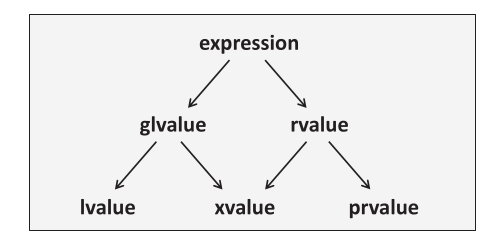
\includegraphics{../imgs/5.1.png}
    \caption{从C++11起的值类型体系}
    \label{f5.1}
\end{figure}

\emph{\textbf{lvalue(左值)}}的例子有:
\begin{itemize}[leftmargin=*]
    \item 只含有单个变量、函数(译者:???)或成员的表达式
    \item 只含有字符串字面量的表达式(译者:???)
    \item 内建的一元\texttt{*}运算符(解引用运算符)的结果
    \item 一个返回\emph{lvalue(左值)}引用(\emph{type\&})的函数的返回值
\end{itemize}
\emph{\textbf{prvalue(纯右值)}}的例子有:
\begin{itemize}[leftmargin=*]
    \item 除字符串字面量和用户自定义字面量之外的字面量组成的表达式
    \item 内建的一元\texttt{\&}运算符(取地址运算符)的运算结果
    \item 内建的数学运算符的结果
    \item 一个返回值的函数的返回值
    \item lambda返回值
\end{itemize}
\emph{\textbf{xvalue(到期值)}}的例子有:
\begin{itemize}[leftmargin=*]
    \item 一个返回右值引用(\emph{type\&\&})的函数的返回值
    (尤其是\texttt{std::move()}的返回值)
    \item 把一个对象转换为右值引用的操作的结果
\end{itemize}
简单来讲:
\begin{itemize}[leftmargin=*]
    \item 所有名称都是\emph{lvalue(左值)}。
    \item 所有用作表达式的字符串字面量是\emph{lvalue(左值)}。
    \item 所有其他的字面量(\texttt{4.2, true, nullptr})是\emph{prvalue(纯右值)}。
    \item 所有临时对象(尤其是以值返回的对象)是\emph{prvalue(纯右值)}。
    \item \texttt{std::move()}是一个\emph{xvalue(到期值)}
\end{itemize}
例如:
\begin{lstlisting}
    class X {
    };
    X v;
    const X c;

    void f(const X&);   // 接受任何值类型
    void f(X&&);        // 只接受prvalue和xvalue,但是相比上边的版本是更好的匹配

    f(v);   // 给第一个f()传递了一个可修改lvalue
    f(c);   // 给第一个f()传递了不可修改的lvalue
    f(X()); // 给第二个f()传递了一个prvalue
    f(std::move(v));    // 给第二个f()传递了一个xvalue
\end{lstlisting}
值得强调的一点是严格来讲glvalue(广义左值)、prvalue(纯右值)、xvalue(到期值)是描述表达式的术语
而\emph{不是}描述值的术语(这意味着这些术语其实是误称)。例如,一个变量自身并不是左值,
只含有这个变量的表达式才是左值:
\begin{lstlisting}
    int x = 3;  // 这里,x是一个变量,不是一个左值
    int y = x;  // 这里,x是一个左值
\end{lstlisting}
在第一条语句中,\texttt{3}是一个纯右值,用它初始化了变量(不是左值)\texttt{x}。
在第二条语句中,\texttt{x}是一个左值(该表达式的求值结果指向一个包含有数值\texttt{3}的对象)。
左值\texttt{x}被转换为一个纯右值,然后用来初始化\texttt{y}。

\subsubsection{自从C++17起的值类型体系}
C++17再次明确了值类型体系,现在的值类型体系如\hyperref[f5.2]{图5.2}所示:

\begin{figure}[ht]
    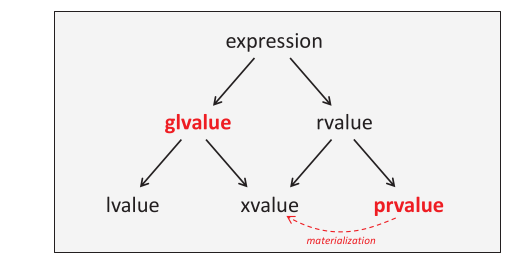
\includegraphics{../imgs/5.2.png}
    \caption{自从C++17起的值类型体系}
    \label{f5.2}
\end{figure}

理解值类型体系的关键是现在广义上来说,我们只有两种类型的表达式:
\begin{itemize}[leftmargin=*]
    \item \textbf{glvaue:} 描述对象或函数\emph{位置}的表达式
    \item \textbf{prvalue:} 用于\emph{初始化}的表达式
\end{itemize}
而\textbf{xvalue}可以认为是一种特殊的位置,它代表一个资源可以被回收利用的对象
(通常是因为该对象的生命周期即将结束)。

C++17引入了一个新的术语:(临时对象的)\emph{实质化}(materialization),
目前prvalue就是一种临时对象。因此,\emph{临时对象实质化转换}
(temporary materialization conversion)是一种prvalue到xvalue的转换。

在任何情况下prvalue出现在需要glvalue(lvalue或者xvalue)的地方都是有效的,
此时会创建一个临时对象并用该prvalue来初始化(注意prvalue主要就是用来初始化的值)。
然后该prvalue会被临时创建的xvalue类型的临时对象替换。因此上面的例子严格来讲是这样的:
\begin{lstlisting}
    void f(const X& p); // 接受一个任何值类型体系的表达式
                        // 但实际上需要一个glvalue
    f(X());             // 传递了一个prvalue,该prvalue实质化为xvalue
\end{lstlisting}
因为这个例子中的\texttt{f()}的形参是一个引用,所以它需要glvaue类型的实参。
然而,表达式\texttt{X()}是一个prvalue。此时“临时变量实质化”规则会产生作用,
表达式\texttt{X()}会“转换为”一个xvalue类型的临时对象。

注意实质化的过程中并没有创建新的/不同的对象。左值引用\texttt{p}仍然\emph{绑定到}
xvalue和prvalue,尽管后者现在会转换为一个xvalue。

因为prvalue不再是对象而是可以被用来初始化对象的表达式,
所以当使用prvalue来初始化对象时不再需要prvalue是可移动的,
进而省略临时变量拷贝的特性可以完美实现。
我们现在只需要简单的传递初始值,然后它会被自动实质化来初始化新对象。
\footnote{感谢Richard Smith和Graham Haynes指出这一点}

\subsection{未实质化的返回值传递}
所有以值返回临时对象(prvalue)的过程都是在传递未实质化的返回值:
\begin{itemize}[leftmargin=*]
    \item 当我们返回一个非字符串字面量的字面量时:
    \begin{lstlisting}
    int f1() {  // 以值返回int
        return 42;
    }
    \end{lstlisting}
    \item 当我们用\texttt{auto}或类型名作为返回类型并返回一个临时对象时:
    \begin{lstlisting}
    auto f2() { // 以值返回退化的类型
        ...
        return MyType{...};
    }
    \end{lstlisting}
    \item 当使用\texttt{decltype(auto)}作为返回类型并返回临时对象时:
    \begin{lstlisting}
    decltype(auto) f3() {   // 返回语句中以值返回临时对象
        ...
        return MyType{...}
    }
    \end{lstlisting}
\end{itemize}

注意当用来初始化的表达式(此处是返回语句)是一个创建临时对象(prvalue)的表达式时
\texttt{decltype(auto)}将会推导出值类型。因为我们在这些场景中都是以值返回一个prvalue,
所以我们完全不需要任何拷贝/移动。

\subsection{后记}
用临时变量初始化时强制省略拷贝由Richard Smith在\url{https://wg21.link/p0135r0}中首次提出。
最终被接受的正式提案由Richard Smith发表于\url{https://wg21.link/p0135r1}。
    \section{lambda表达式扩展}\label{ch6}
lambda表达式是一个很大的成功,它最早在C++11中引入,在C++14中又引入了泛型lambda。
它允许我们将函数作为参数传递,这让我们能更轻易的指明一种行为。

C++17扩展了lambda表达式的应用场景:
\begin{itemize}[leftmargin=*]
    \item 在常量表达式中使用(也就是在编译期间使用)
    \item 在需要当前对象的拷贝时使用(例如,当在不同的线程中调用lambda时)
\end{itemize}

\subsection{\texttt{constexpr} lambda}
自从C++17起,lambda表达式会尽可能的隐式声明\texttt{constexpr}。
也就是说,任何只使用有效的编译期上下文
(例如,只有字面量,没有静态变量,没有虚函数,没有\texttt{try/catch},
没有\texttt{new/delete}的上下文)的lambda都可以被用于编译期。

例如,你可以使用一个lambda表达式计算参数的平方,并将结果用作\texttt{std::array<>}的大小,
即使这是一个编译期的参数:
\begin{lstlisting}
    auto squared = [](auto val) {   // 自从C++17起隐式constexpr
        return val*val;
    };
    std::array<int, squared(5)> a;  // 自从C++17起OK => std::array<int, 25>
\end{lstlisting}
使用\texttt{constexpr}中不允许的特性将会使lambda失去成为\texttt{constexpr}的能力,
不过你仍然可以在运行时上下文中使用lambda:
\begin{lstlisting}
    auto squared2 = [](auto val) {  // 自从C++17起隐式constexpr
        static int calls = 0;   // OK,但会使该lambda不能成为constexpr
        ...
        return val*val;
    };
    std::array<int, squared2(5)> a;     // ERROR:在编译期上下文中使用了静态变量
    std::cout << squared2(5) << '\n';   // OK
\end{lstlisting}
为了确定一个lambda是否能用于编译期,你可以将它声明为\texttt{constexpr}:
\begin{lstlisting}
    auto squared3 = [](auto val) constexpr {    // 自从C++17起OK
        return val*val;
    };
\end{lstlisting}
如果指明返回类型的话,看起来像下面这样:
\begin{lstlisting}
    auto squared3i = [](int val) constexpr -> int {    // 自从C++17起OK
        return val*val;
    };
\end{lstlisting}
关于\texttt{constexpr}函数的规则也适用于lambda:如果一个lambda在运行时上下文中使用,
那么相应的函数体也会在运行时才会执行。

然而,如果在声明了\texttt{constexpr}的lambda内使用了编译期上下文中不允许出现的特性
将会导致编译错误:\footnote{不允许出现在编译期上下文中的特性有:静态变量、虚函数、
\texttt{try/catch}、\texttt{new/delete}等。}
\begin{lstlisting}
    auto squared4 = [](auto val) constexpr {
        static int calls = 0;   // ERROR:在编译期上下文中使用了静态变量
        ...
        return val*val;
    };
\end{lstlisting}
一个隐式或显式的\texttt{constexpr} lambda的函数调用符也是\texttt{constexpr}。
也就是说,如下定义:
\begin{lstlisting}
    auto squared = [](auto val) {   // 自从C++17起隐式constexpr
        return val*val;
    };
\end{lstlisting}
将会被转换为如下\emph{闭包类型}(closure type):
\begin{lstlisting}
    class CompilerSpecificName {
      public:
        ...
        template<typename T>
        constexpr auto operator() (T val) const {
            return val*val;
        }
    };
\end{lstlisting}
注意,这里自动生成的闭包类型的函数调用运算符自动声明为\texttt{constexpr}。
自从C++17起,如果lambda被显式或隐式地定义为\texttt{constexpr},
那么生成的函数调用运算符将自动是\texttt{constexpr}。
注意如下定义:
\begin{lstlisting}
    auto squared1 = [](auto val) constexpr {    // 编译期lambda调用
        return val*val;
    };
\end{lstlisting}
和如下定义:
\begin{lstlisting}
    constexpr auto squared2 = [](auto val) {    // 编译期初始化squared2
        return val*val;
    };
\end{lstlisting}
是不同的。\\
第一个例子中如果(只有)lambda是\texttt{constexpr}那么它可以被用于编译期,
但是\texttt{squared1}可能直到运行期才会被初始化,
这意味着如果静态初始化顺序很重要那么可能导致问题。
如果用lambda初始化的闭包对象是\texttt{constexpr},那么该对象将在程序开始时就初始化,
但lambda可能还是只能在运行时使用。因此,可以考虑使用如下定义:
\begin{lstlisting}
    constexpr auto squared = [](auto val) constexpr {
        return val*val;
    };
\end{lstlisting}

\subsubsection{使用\texttt{constexpr} lambda}
这里有一个使用\texttt{constexpr} lambda的例子。
假设我们有一个字符串的哈希函数,这个函数迭代字符串的每一个字符反复更新哈希值:
\footnote{djb2算法的源码见\url{http://www.cse.yorku.ca/~oz/hash.html}。}
\begin{lstlisting}
    auto hashed = [](const char* str) {
        std::size_t hash = 5381;    // 初始化哈希值
        while (*str != '\0') {
            hash = hash * 33 ^ *str++;  // 根据下一个字符更新哈希值
        }
        return hash;
    };
\end{lstlisting}
使用这个lambda,我们可以在编译期初始化不同字符串的哈希值,并定义为枚举:
\begin{lstlisting}
    enum Hashed { beer = hashed("beer"),
                  wine = hashed("wine"),
                  water = hashed("water"),
                  ... };   // OK,编译期哈希
\end{lstlisting}
我们也可以在编译期计算\texttt{case}标签:
\begin{lstlisting}
    switch (hashed(argv[1])) {  // 运行时哈希
        case hashed("beer"):    // OK,编译期哈希
            ...
            break;
        case hashed("wine"):
            ...
            break;
        ...
    }
\end{lstlisting}
注意这里我们在编译期调用\texttt{case}标签里的\texttt{hashed},
而在运行期间调用\texttt{switch}表达式里的\texttt{hashed}。

如果我们使用编译期lambda初始化一个容器,那么编译器优化时很可能在编译期就计算出容器的初始值
(这里使用了\hyperref[ch9.2.6.3]{\texttt{std::array}的类模板参数推导}):
\begin{lstlisting}
    std::array arr{ hashed("beer"),
                    hashed("wine"),
                    hashed(("water")};
\end{lstlisting}
你甚至可以在\texttt{hashed}里联合使用另一个\texttt{constexpr} lambda。
设想我们把\texttt{hashed}里根据当前哈希值和下一个字符值更新哈希值的逻辑定义为一个参数:
\begin{lstlisting}
    auto hashed = [](const char* str, auto combine) {
        std::size_t hash = 5381;
        while (*str != '\0') {
            hash = combine(hash, *str++);   // 用下一个字符更新哈希值
        }
        return hash;
    };
\end{lstlisting}
这个lambda可以像下面这样使用:
\begin{lstlisting}
    constexpr std::size_t hv1{
        hashed("wine"), [](auto h, char c) {return h*33 + c;})};
    constexpr std::size_t hv2{
        hashed("wine"), [](auto h, char c) {return h*33 ^ c;})};
\end{lstlisting}
这里,我们在编译期通过改变更新逻辑初始化了两个不同的"wine"的哈希值。
两个\texttt{hashed}都是在编译期调用。

\subsection{向lambda传递\texttt{this}的拷贝}
当在非静态成员函数里使用lambda时,你不能隐式获取对该对象成员的使用权。
也就是说,如果你不捕获\texttt{this}的话你将不能在lambda里使用该对象的任何成员
(即使你用\texttt{this->}来访问也不行):
\begin{lstlisting}
    class C {
      private:
        std::string name;
      public:
        ...
        void foo() {
            auto l1 = [] {std::cout << name << '\n';}; // ERROR
            auto l2 = [] {std::cout << this->name << '\n';}; // ERROR
            ...
        }
    };
\end{lstlisting}
在C++11和C++14里,你可以通过值或引用捕获\texttt{this}:
\begin{lstlisting}
    class C {
      private:
        std::string name;
      public:
        ...
        void foo() {
            auto l1 = [this] {std::cout << name << '\n';}; // OK
            auto l2 = [=] {std::cout << name << '\n';}; // OK
            auto l3 = [&] {std::cout << name << '\n';}; // OK
            ...
        }
    };
\end{lstlisting}
然而,问题是即使是用拷贝的方式捕获\texttt{this}实质上获得的也是引用
(因为只会拷贝\texttt{this}指针)。当lambda的生命周期比该对象的生命周期更长的时候,
调用这样的函数就可能导致问题。比如一个极端的例子是在lambda中开启一个新的线程来完成某些任务,
调用新线程时正确的做法是传递整个对象的拷贝来避免并发和生存周期的问题,而不是传递该对象的引用。
另外有时候你可能只是简单的想向lambda传递当前对象的拷贝。

自从C++14起有了一个解决方案,但可读性和实际效果都比较差:
\begin{lstlisting}
    class C {
      private:
        std::string name;
      public:
        ...
        void foo() {
            auto l1 = [thisCopy=*this] { std::cout << thisCopy.name << '\n'; };
            ...
        }
    };
\end{lstlisting}
例如,当使用了\texttt{=}或者\texttt{\&}捕获了其他对象的时候你可能会在不经意间使用\texttt{this}:
\begin{lstlisting}
    auto l1 = [&, thisCopy=*this] {
        thisCopy.name = "new name";
        std::cout << name << '\n'; // OOPS:仍然使用了原来的name
    };
\end{lstlisting}
自从C++17起,你可以通过\texttt{*this}显式地捕获当前对象的拷贝:
\begin{lstlisting}
    class C {
      private:
        std::string name;
      public:
        ...
        void foo() {
            auto l1 = [*this] { std::cout << name << '\n'; };
            ...
        }
    };
\end{lstlisting}
这里,捕获\texttt{*this}意味着该lambda生成的闭包将存储当前对象的一份\emph{拷贝}。

你仍然可以在捕获\texttt{*this}的同时捕获其他对象,只要没有多个\texttt{this}的矛盾:
\begin{lstlisting}
    auto l2 = [&, *this] { ... };       // OK
    auto l3 = [this, *this] { ... };    // ERROR
\end{lstlisting}
这里有一个完整的例子:
\begin{lstlisting}[frame=single, title=lang/lambdathis.cpp]
    #include <iostream>
    #include <string>
    #include <thread>

    class Data {
      private:
        std::string name;
      public:
        Data(const std::string& s) : name(s) {
        }
        auto startThreadWithCopyOfThis() const {
            // 开启并返回新线程,新线程将在3秒后使用this
            using namespace std::literals;
            std::thread t([*this] {
                std::this_thread::sleep_for(3s);
                std::cout << name << '\n';
            });
            return t;
        }
    };

    int main()
    {
        std::thread t;
        {
            Data d{"c1"};
            t = d.startThreadWithCopyOfThis();
        }   // d不再有效
        t.join();
    }
\end{lstlisting}
lambda里捕获了\texttt{*this},因此传递进lambda的是一份拷贝。
因此,即使在\texttt{d}被销毁之后使用捕获的对象也没有问题。

如果我们使用\texttt{[this]}、\texttt{[=]}或者\texttt{[\&]}捕获\texttt{this},
那么新线程将会陷入未定义行为,因为当线程中打印\texttt{name}的时候将会使用一个已经销毁的
对象的成员。

\subsection{以常量引用捕获}
通过使用一个新的库工具,现在也可以\nameref{ch25.2.1}。

\subsection{后记}
\texttt{constexpr} lambda最早由Faisal Vali、Ville Voutilainen、Gabriel Dos Reis
在\url{https://wg21.link/n4487}中首次提出。
最终被接受的正式提案由Faisal Vali、Jens Maurer、Richard Smith
发表于\url{https://wg21.link/p0170r1}。
    \section{新属性和属性特性}\label{ch7}
自从C++11起,就可以指明\emph{属性}(attribute)(允许或者禁用某些警告的注解)。
C++17引入了新的属性,另外现在属性也可以在其他一些地方使用,也许能带来一些便利。

\subsection{\texttt{[[nodiscard]]}属性}
新属性\texttt{[[nodiscard]]}可以鼓励编译器在某个函数的返回值未被使用时给出警告
(这并不意味着编译器一定要给出警告)。
\texttt{[[nodiscard]]}通常应该用于防止某些因为返回值未被使用导致的不当行为。
这些不当行为可能是(译者注:请配合下边的例子理解这些不当行为):
\begin{itemize}[leftmargin=*]
    \item \textbf{内存泄露},例如返回值中含有动态分配的内存,但并未使用。
    \item \textbf{未知的或出乎意料的行为},例如因为没有使用返回值而导致了一些奇怪的行为。
    \item \textbf{不必要的开销},例如因为返回值没被使用而进行了一些无意义的行为。
\end{itemize}
这里有一些该属性发挥所用的例子:
\begin{itemize}[leftmargin=*]
    \item 申请资源但自身并不释放,而是将资源返回等待其他函数释放的函数应该被标记为
    \texttt{[[nodiscard]]}。一个典型的例子是申请内存的函数,
    例如\texttt{malloc()}函数或者分配器的\texttt{allocate()}成员函数。

    然而,注意有些函数\emph{可能}会返回一个无需再处理的值。例如,程序员可能会用0字节调用C函数
    \texttt{realloc()}来释放内存,这种情况下的返回值无需之后调用\texttt{free()}函数释放。
    因此,如果对\texttt{realloc()}标记\texttt{[[nodiscard]]}将会适得其反。
    \item 有时如果没有使用返回值将导致函数行为和预期不同,一个很好的例子是\texttt{std::async()}
    (C++11引入)。\texttt{std::async()}会在后台异步地执行一个任务并返回一个可以用来等待
    任务执行结束的句柄(也可以通过它获取返回值或者异常)。然而,如果返回值没有被使用的话该调用
    将变成同步的调用,因为在启动任务的语句结束之后未被使用的返回值的析构函数会立即执行,而析构
    函数会阻塞等待任务运行结束。因此,不使用返回值导致的结果与\texttt{std::async()}的目的
    完全矛盾。将\texttt{std::async()}标记为\texttt{[[nodiscard]]}可以让编译器给出警告。
    \item 另一个例子是成员函数\texttt{empty()},它的作用是检查一个对象(容器/字符串)是否
    没有元素。程序员经常误用该函数来“清空“容器:
    \begin{lstlisting}
    cont.empty();
    \end{lstlisting}
    这种对\texttt{empty()}的误用并没有使用返回值,所以\texttt{[[nodiscard]]}可以检查出这种误用:
    \begin{lstlisting}
    class MyContainer {
        ...
      public:
        [[nodiscard]] bool empty() const noexcept;
        ...
    };
    \end{lstlisting}
    这里的属性标记可以帮助检查这种逻辑错误。
\end{itemize}
如果因为某些原因你不想使用一个被标记为\texttt{[[nodiscard]]}的函数的返回值,
你可以把返回值转换为\texttt{void}:
\begin{lstlisting}
    (void)coll.empty(); // 禁止[[nodiscard]]警告
\end{lstlisting}
注意如果成员函数被覆盖或者隐藏时基类中标记的属性不会被继承:
\begin{lstlisting}
    struct B {
        [[nodiscard]] int* foo();
    };

    struct D : B {
        int* foo();
    };

    B b;
    b.foo();        // 警告
    (void)b.foo();  // 没有警告

    D d;
    d.foo();        // 没有警告
\end{lstlisting}
因此你需要给派生类里相应的成员函数再次标记\texttt{[[nodiscard]]}
(除非有某些原因导致你不想在派生类里确保返回值必须被使用)。

你可以把属性标记在函数前的所有修饰符之前,也可以标记在函数名之后:
\begin{lstlisting}
    class C {
        ...
        [[nodiscard]] friend bool operator== (const C&, const C&);
        friend bool operator!= [[nodiscard]] (const C&, const C&);
    };
\end{lstlisting}
把属性放在\texttt{friend}和\texttt{bool}之间或者\texttt{bool}和\texttt{operator==}
之间是错误的。

尽管这个特性从C++17起引入,但它还没有在标准库中使用。因为这个提案出现的太晚了,所以最应该
需要它的\texttt{std::async()}也还没有使用它。不过这里讨论的所有例子,将在下一次C++标准
中实现(见C++20中通过的\url{https://wg21.link/p0600r1}提案)。

为了保证代码的可移植性,你应该使用\texttt{[[nodiscard]]}而不是一些不可移植的方案
(例如gcc和clang的\texttt{[[gnu:warn\_unused\_result]]}或者Visual C++的
\texttt{\_Check\_return\_})。

当\hyperref[ch30.2.2]{定义\texttt{new()}运算符}时,
你应该用\texttt{[[nodiscard]]}对该函数进行标记,
例如\hyperref[ch30.4]{定义一个追踪所有\texttt{new}调用的头文件}。

\subsection{\texttt{[[maybe\_unused]]}属性}
新的属性\texttt{[[maybe\_unused]]}可以避免编译器在某个变量未被使用时发出警告。
新的属性可以应用于类的声明、使用\texttt{typedef}或者\texttt{using}定义的类型、
一个变量、一个非静态数据成员、一个函数、一个枚举类型、一个枚举值等场景。

例如其中一个作用是定义一个可能不会使用的参数:
\begin{lstlisting}
    void foo(int val, [[maybe_unused]] std::string msg)
    {
    #ifdef DEBUG
        log(msg);
    #endif
        ...
    }
\end{lstlisting}
另一个例子是定义一个可能不会使用的成员:
\begin{lstlisting}
    class MyStruct {
        char c;
        int i;
        [[maybe_unused]] char makeLargerSize[100];
        ...
    };
\end{lstlisting}
注意你不能在一条语句上应用\texttt{[[maybe\_unused]]}。
也就是说,你不能直接用\texttt{[[maybe\_unused]]}来抵消\texttt{[[nodiscard]]}的作用:
\footnote{感谢Roland Bock指出这一点}
\begin{lstlisting}
    [[nodiscard]] void* foo();
    int main()
    {
        foo();  // 警告:返回值没有使用
        [[maybe_unused]] foo(); // 错误:maybe_unused不允许出现在此
        [[maybe_unused]] auto x = foo(); // OK
    }
\end{lstlisting}

\subsection{\texttt{[[fallthrough]]}属性}
新的属性\texttt{[[fallthrough]]}可以避免编译器在\texttt{switch}语句中某一个标签
缺少\texttt{break}语句时发出警告。例如:
\begin{lstlisting}
    void commentPlace(int place)
    {
        switch (place) {
            case 1:
                std::cout << "very ";
                [[fallthrough]];
            case 2:
                std::cout << "well\n";
                break;
            default:
                std::cout << "OK\n";
                break;
        }
    }
\end{lstlisting}
这个例子中参数为1时将输出:
\begin{lstlisting}
    very well
\end{lstlisting}
\texttt{case 1}和\texttt{case 2}中的语句都会被执行。
注意这个属性必须被用作单独的语句,还要有分号结尾。
另外在\texttt{switch}语句的最后一个分支不能使用它。

\subsection{通用的属性扩展}
自从C++17起下列有关属性的通用特性变得可用:
\begin{enumerate}[leftmargin=*]
    \item 属性现在可以用来标记命名空间。例如,你可以像下面这样弃用一个命名空间:
    \begin{lstlisting}
    namespace [[deprecated]] DraftAPI {
        ...
    }
    \end{lstlisting}
    这也可以应用于内联的和匿名的命名空间。
    \item 属性现在可以标记枚举子(枚举类型的值)。
    例如你可以像下面这样引入一个新的枚举值作为某个已有枚举值(并且现在已经被废弃)的替代:
    \begin{lstlisting}
    enum class City { Berlin = 0,
        NewYork = 1,
        Mumbai = 2,
        Bombay [[deprecated]] = Mumbai,
        ... };
    \end{lstlisting}
    这里\texttt{Mumbai}和\texttt{Bombay}代表同一个城市的数字码,但使用\texttt{Bombay}
    已经被标记为废弃的。注意对于枚举值,属性被放置在标识符\emph{之后}。
    \item 用户自定义的属性一般应该定义在自定义的命名空间中。现在可以使用\texttt{using}前缀
    来避免为每一个属性重复输入命名空间。也就是说,如下代码:
    \begin{lstlisting}
    [[MyLib::WebService, MyLib::RestService, MyLib::doc("html")]] void foo();
    \end{lstlisting}
    可以被替换为
    \begin{lstlisting}
    [[using MyLib: WebService, RestService, doc("html")]] void foo();
    \end{lstlisting}
    注意在使用了\texttt{using}前缀时重复命名空间将导致错误:
    \begin{lstlisting}
    [[using MyLib: MyLib::doc("html")]] void foo(); // ERROR
    \end{lstlisting}
\end{enumerate}

\subsection{后记}
三个新属性由Andrew Tomazos在\url{https://wg21.link/p0068r0}中首次提出。

\texttt{[[nodiscard]]}最终被接受的提案由Andrew Tomazos发表于
\url{https://wg21.link/p0189r1}。

\texttt{[[maybe\_unused]]}最终被接受的提案由Andrew Tomazos发表于
\url{https://wg21.link/p0212r1}。

\texttt{[[fallthrough]]}最终被接受的提案由Andrew Tomazos发表于
\url{https://wg21.link/p0188r1}。

允许为命名空间和枚举值标记属性的特性由Richard Smith在\url{https://wg21.link/n4196}
中首次提出。该特性最终被接受的提案由Richard Smith发表于\url{https://wg21.link/n4266}。

属性的\texttt{using}前缀由J. Daniel Garcia、Luis M. Sanchez、
Massimo Torquati、Marco Danelutto、Peter Sommerlad在\url{https://wg21.link/p0028r0}
中首次提出。最终被接受的提案由J. Daniel Garcia和Daveed Vandevoorde发表于
\url{https://wg21.link/P0028R4}。


    \part{模板特性}\label{part2}
    这一部分介绍了C++17为泛型编程(即template)提供的新的语言特性。

    我们首先从类模板参数推导开始,这一特性只影响模板的使用。之后的章节会介绍为编写泛型代码(函数模板,
    类模板,泛型库等)的程序员提供的新特性。

    \section{类模板参数推导}\label{ch9}
在C++17之前,你必须明确指出类模板的所有参数。
例如,你不可以省略下面的\texttt{double}:
\begin{lstlisting}
    std::complex<double> c{5.1, 3.3};
\end{lstlisting}
也不可以省略下面的\texttt{std::mutex}:
\begin{lstlisting}
    std::mutex mx;
    std::lock_guard<std::mutex> lg(mx);
\end{lstlisting}
自从C++17起必须指明类模板参数的限制被放宽了。
通过使用\emph{类模板参数推导}(class template argument deduction)(CTAD),
只要编译器能根据初始值\emph{推导出}所有模板参数,那么就可以不指明参数。

例如:
\begin{itemize}[leftmargin=*]
    \item 你现在可以这么声明:
    \begin{lstlisting}
    std::complex c{5.1, 3.3};   // OK:推导出std::complex<double>
    \end{lstlisting}
    \item 你现在可以这么写:
    \begin{lstlisting}
    std::mutex mx;
    std::lock_guard lg{mx}; // OK:推导出std::lock_guard<std::mutex>
    \end{lstlisting}
    \item 你现在甚至可以让容器来推导元素类型:
    \begin{lstlisting}
    std::vector v1{1, 2, 3}; // OK:推导出std::vector<int>
    std::vector v2{"hello", "world"}; // OK:推导出std::vector<const char*>
    \end{lstlisting}
\end{itemize}

\subsection{使用类模板参数推导}
只要能根据初始值推导出所有模板参数就可以使用类模板参数推导。
推导过程支持所有方式的初始化(只要保证初始化是有效的):
\begin{lstlisting}
    std::complex c1{1.1, 2.2};  // 推导出std::complex<double>
    std::complex c2(2.2, 3.3);  // 推导出std::complex<double>
    std::complex c3 = 3.3;      // 推导出std::complex<double>
    std::complex c4 = {4.4};    // 推导出std::complex<double>
\end{lstlisting}
因为\texttt{std::complex}只需要一个参数就可以初始化并推导出模板参数\texttt{T}:
\begin{lstlisting}
    namespace std {
        template<typename T>
        class complex {
            constexpr complex(const T&re = T(), const T& im = T());
            ...
        }
    };
\end{lstlisting}
所以\texttt{c3}和\texttt{c4}可以正确初始化。
对于如下声明:
\begin{lstlisting}
    std::complex c1{1.1, 2.2};
\end{lstlisting}
编译器会查找到构造函数:
\begin{lstlisting}
    constexpr complex(const T& re = T(), const T& im = T());
\end{lstlisting}
并调用。因为两个参数都是\texttt{double}类型,因此编译器会推导出\texttt{T}的就是
\texttt{double}并生成如下代码:
\begin{lstlisting}
    complex<double>::complex(const double& re = double(),
                             const double& im = double());
\end{lstlisting}
注意推导的过程中模板参数必须没有歧义。也就是说,如下初始化代码不能通过编译:
\begin{lstlisting}
    std::complex c5{5, 3.3};    // ERROR:尝试将T推导为int和double
\end{lstlisting}
推导模板参数时不会使用隐式类型转换。

也可以对可变参数模板使用类模板参数推导。例如,对于一个如下定义的\texttt{std::tuple}:
\begin{lstlisting}
    namespace std {
        template<typename... Types>
        class tuple {
          public:
            constexpr tuple(const Types&...);
            ...
        };
    };
\end{lstlisting}
如下声明:
\begin{lstlisting}
    std::tuple t{42, 'x', nullptr};
\end{lstlisting}
将推导出类型\texttt{std::tuple<int, char, std::nullptr\_t>}。

你也可以推导非类型模板参数。
例如,我们可以根据传入的参数同时推导数组的元素类型和元素数量:
\begin{lstlisting}
    template<typename T, int SZ>
    class MyClass {
      public:
        MyClass (T(&)[SZ]) {
            ...
        }
    };

    MyClass mc("hello");    // 推导出T为const char,SZ为6
\end{lstlisting}
这里我们推导出\texttt{SZ}为\texttt{6}因为传入的字符串字面量有6个字符。
\footnote{注意构造函数里以引用作为参数是必须的。
否则根据语言规则传入的字符数组将会退化为指针,然后将无法推导出\texttt{SZ}。}

你甚至可以推导\hyperref[ch14.1]{用作基类的lambda}来实现重载
或者推导\hyperref[ch13.1]{\texttt{auto}模板参数}。

\subsubsection{默认以拷贝方式推导}\label{ch9.1.1}
类模板参数推导过程中会首先尝试以拷贝的方式初始化。
例如,首先初始化一个只有一个元素的\texttt{std::vector}:
\begin{lstlisting}
    std::vector v1{42}; // 一个元素的vector<int>
\end{lstlisting}
然后使用这个vector初始化另一个vector,推导时会解释为创建一个拷贝:
\begin{lstlisting}
    std::vector v2{v1}; // v2也是一个std::vector<int>
\end{lstlisting}
而不是创建一个只有一个元素的\texttt{vector<vector<int>>}。

这个规则适用于所有形式的初始化:
\begin{lstlisting}
    std::vector v2{v1};         // v2也是vector<int>
    std::vector v3(v1);         // v3也是vector<int>
    std::vector v4 = {v1};      // v4也是vector<int>
    auto v5 = std::vector{v1};  // v5也是vector<int>
\end{lstlisting}
注意这是花括号初始化总是把列表中的参数作为元素这一规则的一个例外。
如果你传递一个只有一个vector的初值列来初始化另一个vector,
你将得到一个传入的vector的拷贝。然而,如果用多于一个元素的初值列来初始化的话
就会把传入的参数作为元素并推导出其类型作为模板参数(因为这种情况下无法解释为创建拷贝):
\begin{lstlisting}
    std::vector vv{v1, v2}; // vv是一个vector<vector<int>>
\end{lstlisting}
这引出了一个问题就是对可变参数模板使用类模板参数推导时会发生什么:
\begin{lstlisting}
    template<typename... Args>
    auto make_vector(const Args&... elems) {
        return std::vector{elem...};
    }

    std::vector<int> v{1, 2, 3};
    auto x1 = make_vector(v, v);    // vector<vector<int>>
    auto x2 = make_vector(v);       // vector<int>还是vector<vector<int>>?
\end{lstlisting}
目前不同的编译器会有不同的行为,这个问题还在讨论之中。

\subsubsection{推导lambda的类型}
通过使用类模板参数推导,我们可以用lambda的类型(确切的说是lambda生成的\emph{闭包}的类型)
作为模板参数来实例化类模板。例如我们可以提供一个泛型类,对一个任意回调函数进行包装并统计调用次数:
\begin{lstlisting}[frame=single, title=tmpl/classarglambda.hpp]
    #include <utility>  // for std::forward()

    template<typename CB>
    class CountCalls
    {
      private:
        CB callback;    // 要调用的回调函数
        long calls = 0; // 调用的次数
      public:
        CountCalls(CB cb) : callback(cb) {
        }
        template<typename... Args>
        decltype(auto) operator() (Args&&... args) {
            ++calls;
            return callback(std::forward<Args>(args)...);
        }
        long count() const {
            return calls;
        }
    };
\end{lstlisting}
这里构造函数获取一个回调函数并进行包装,这样在初始化时会把参数的类型推导为\texttt{CB}。
例如,我们可以使用一个lambda作为参数来初始化一个对象:
\begin{lstlisting}
    CountCalls sc{[](auto x, auto y) {
                    return x > y;
                }};
\end{lstlisting}
这意味着排序准则\texttt{sc}的类型将被推导为\texttt{CountCalls<}\emph{TypeOfTheLambda}
\texttt{>}。这样,我们可以统计出排序准则被调用的次数:
\begin{lstlisting}
    std::sort(v.begin(), v.end(),   // 排序区间
                std::ref(sc));  // 排序准则
    std::cout << "sorted with " << sc.count() << " calls\n";
\end{lstlisting}
这里,包装过后的lambda被用作排序准则。注意必须要传递引用,否则\texttt{std::sort()}将会
获取\texttt{sc}的拷贝作为参数,计数时只会修改该拷贝内的计数器。

然而,我们可以直接把包转后的lambda传递给\texttt{std::for\_each()},
因为该算法(非并行版本)最后会返回传入的回调函数,以便于获取回调函数最终的状态:
\begin{lstlisting}
    auto fo = std::for_each(v.begin(), v.end(),
                    CountCalls{[](auto i) {
                        std::cout << "elem: " << i << '\n';
                    }});
    std::cout << "output with " << fo.count() << " calls\n";
\end{lstlisting}
输出将会如下(排序准则调用次数可能会不同,因为\texttt{sort()}的实现可能会不同):
\begin{lstlisting}
    sorted with 39 calls
    elem: 19
    elem: 17
    elem: 13
    elem: 11
    elem: 9
    elem: 7
    elem: 5
    elem: 3
    elem: 2
    output with 9 calls
\end{lstlisting}
如果计数器是原子的,你也可以使用\hyperref[ch22]{并行算法}:
\begin{lstlisting}
    std::sort(std::execution::par,
                v.begin(), v.end(),
                std::ref(sc));
\end{lstlisting}

\subsubsection{没有类模板部分参数推导}
注意,不像函数模板,类模板不能只指明一部分模板参数,然后指望编译器去推导剩余的部分参数。
甚至使用\texttt{<>}指明空模板参数列表也是不允许的。例如:
\begin{lstlisting}
    template<typename T1, typename T2, typename T3 = T2>
    class C
    {
      public:
        C (T1 x = {}, T2 y = {}, T3 z = {}) {
            ...
        }
        ...
    };

    // 推导所有参数
    C c1(22, 44.3, "hi");   // OK:T1是int,T2是double,T3是const char*
    C c2(22, 44.3);     // OK:T1是int,T2和3是double
    C c3("hi", "guy");  // OK:T1、T2、T3都是const char*

    // 推导部分参数
    C<string> c4("hi", "my");   // ERROR:只有T1显式指明
    C<> c5(22, 44.3);           // ERROR:T1和T2都没有指明
    C<> c6(22, 44.3, 42);       // ERROR:T1和T2都没有指明

    // 指明所有参数
    C<string, string, int> c7;   // OK:T1、T2是string,T3是int
    C<int, string> c8(52, "my"); // OK:T1是int,T2、T3是string
    C<string, string> c9("a", "b", "c");    // OK:T1、T2、T3都是string
\end{lstlisting}
注意第三个模板参数有默认值,因此只要指明了第二个参数就不需要再指明第三个参数。

如果你想知道为什么不支持部分参数推导,这里有一个导致这个决定的例子:
\begin{lstlisting}
    std::tuple<int> t(42, 43);  // 仍然ERROR
\end{lstlisting}
\texttt{std::tuple}是一个可变参数模板,因此你可以指明任意数量的模板参数。
在这个例子中,并不能判断出只指明一个参数是一个错误还是故意的。

不幸的是,不支持部分参数推导意味着一个常见的编码需求并没有得到解决。
我们仍然不能简单的使用一个lambda作为关联容器的排序准则或者无序容器的hash函数:
\begin{lstlisting}
    std::set<Cust> coll([] (const Cust& x, const Cust& y) { // 仍然ERROR
                            return x.getName() > y.getName();
                        });
\end{lstlisting}
我们仍然不得不指明lambda的类型。例如:
\begin{lstlisting}
    auto sortcrit = [](const Cust& x, const Cust& y) {
                        return x.getName() > y.getName();
                    };
    std::set<Cust, decltype(sortcrit)> coll(sortcrit); // OK
\end{lstlisting}
仅仅指明类型是不行的,因为容器初始化时会尝试用给出的lambda类型创建一个lambda。
但这在C++17中是不允许的,因为默认构造函数只有编译器才能调用。
在C++20中如果lambda不需要捕获任何东西的话这将成为可能。

\subsubsection{使用类模板参数推导代替快捷函数}\label{ch9.1.4}
原则上讲,通过使用类模板参数推导,我们可以摆脱已有的几个快捷函数模板,
这些快捷函数的作用其实就是根据传入的参数实例化相应的类模板。

一个明显的例子是\texttt{std::make\_pair()},它可以帮助我们避免指明传递进入的参数的类型。
例如,在如下声明之后:
\begin{lstlisting}
    std::vector<int> v;
\end{lstlisting}
我们可以这样:
\begin{lstlisting}
    auto p = std::make_pair(v.begin(), v.end());
\end{lstlisting}
而不需要写:
\begin{lstlisting}
    std::pair<typename std::vector<int>::iterator,
              typename std::vector<int>::iterator> p(v.begin(), v.end());
\end{lstlisting}
现在这种场景已经不再需要\texttt{std::make\_pair()}了,我们可以简单的写为:
\begin{lstlisting}
    std::pair p(v.begin(), v.end());
\end{lstlisting}
或者:
\begin{lstlisting}
    std::pair p{v.begin(), v.end());
\end{lstlisting}

然而,从另一个角度来看\texttt{std::make\_pair()}也是一个很好的例子,
它演示了有时便捷函数的作用不仅仅是推导模板参数。
事实上,\texttt{std::make\_pair()}会使传入的参数退化
(在C++03中以值传递,自从C++11起使用特征)。
这样会导致字符串字面量的类型(字符数组)会被推导为\texttt{const char*}:
\begin{lstlisting}
    auto q = std::make_pair("hi", "world"); // 推导为指针的pair
\end{lstlisting}
这个例子中,\texttt{q}的类型为\texttt{std::pair<const char*, const char*>}。

使用类模板参数推导会让事情变得更加复杂。
请看下面这个类似于\texttt{std::pair}的简单的类的声明:
\begin{lstlisting}
    template<typename T1, typename T2>
    struct Pair1 {
        T1 first;
        T2 second;
        Pair1(const T1& x, const T2& y) :
            first{x}, second{y} { }
    };
\end{lstlisting}
这里元素以引用传入,根据语言规则,当以引用传递参数时模板参数的类型不会退化。
因此,当调用:
\begin{lstlisting}
    Pair1 p1{"hi", "world"}; // 推导为不同大小的数组的pair,但是……
\end{lstlisting}
\texttt{T1}被推导为\texttt{char[3]},\texttt{T2}被推导为\texttt{char[6]}。
原则上讲这样的推导是有效的。然而,我们使用了\texttt{T1}和\texttt{T2}来声明成员
\texttt{first}和\texttt{second},因此它们被声明为:
\begin{lstlisting}
    char first[3];
    char second[6];
\end{lstlisting}
然而使用一个左值数组来初始化另一个数组是不允许的。它类似于尝试编译如下代码:
\begin{lstlisting}
    const char x[3] = "hi";
    const char y[6] = "world";
    char first[3] {x};  // ERROR
    char second[6] {y}; // ERROR
\end{lstlisting}
注意如果我们声明参数时以值传参就不会再有这个问题:
\begin{lstlisting}
    tempalte<typename T1, typename T2>
    struct Pair2 {
        T1 first;
        T2 second;
        Pair2(T1 x, T2 y) :
            first{x}, second{y} { }
    };
\end{lstlisting}
如果我们像下面这样创建新对象:
\begin{lstlisting}
    Pair2 p2{"hi", "world"}; // 推导为指针的pair
\end{lstlisting}
\texttt{T1}和\texttt{T2}都会被推导为\texttt{const char*}。

然而,因为\texttt{std::pair<>}的构造函数以引用传参,
所以下面的初始化正常情况下应该不能通过编译:
\begin{lstlisting}
    std::pair p{"hi", "world"}; // 看似会推导出不同大小的数组的pair,但是……
\end{lstlisting}
然而你,事实上它能通过编译,因为\texttt{std::pair<>}定义\emph{推导指引},
我们将在下一小节讨论它。

\subsection{推导指引}
你可以定义特定的\emph{推导指引}来给类模板参数添加新的推导或者修正构造函数定义的推导。
例如,你可以定义无论何时推导\texttt{Pair3}的模板参数,推导的行为都好像参数是以值传递的:
\begin{lstlisting}
    template<typename T1, typename T2>
    struct Pair3 {
        T1 first;
        T2 second;
        Pair3(const T1& x, const T2& y) :
            first{x}, second{y} { }
    };

    // 为构造函数定义的推导指引
    tempalte<typename T1, typename T2>
    Pair3(T1, T2) -> Pair3<T1, T2>;
\end{lstlisting}
在\texttt{->}的左侧我们声明了我们\emph{想要推导什么}。
这里我们声明的是使用两个以值传递且类型分别为\texttt{T1}和\texttt{T2}的对象
创建一个\texttt{Pair3}对象。
在\texttt{->}的右侧,我们定义了推导的结果。
在这个例子中,\texttt{Pair3}以类型\texttt{T1}和\texttt{T2}实例化。

你可能会说这是构造函数已经做到的事情。
然而,构造函数是以引用传参,两者是不同的。
一般来说,不仅是模板,所有以值传递的参数都会退化,而以引用传递的参数不会退化。
退化意味着原生数组会转换为指针,并且顶层的修饰符例如\texttt{const}或者引用将会被忽略。

如果没有推导指引,对于如下声明:
\begin{lstlisting}
    Pair3 p3{"hi", "world"};
\end{lstlisting}
参数\texttt{x}的类型是\texttt{const char(\&)[3]},因此\texttt{T1}是\texttt{char[3]},
参数\texttt{y}的类型是\texttt{const char(\&)[6]},因此\texttt{T2}是\texttt{char[6]}。

有了推导指引饮后,模板参数就会退化。这意味着传入的数组或者字符串字面量会退化为相应的指针类型。
现在,如下声明:
\begin{lstlisting}
    Pair3 p3{"hi", "world"};
\end{lstlisting}
推导指引会发挥作用,因此会以值传参。因此,两个类型都会退化为\texttt{const char*},
然后被用作模板参数推导的结果。上面的声明和如下声明等价:
\begin{lstlisting}
    Pair3<const char*, const char*> p3{"hi", "world"};
\end{lstlisting}
注意构造函数仍然以引用传参。推导指引只和模板参数的推导相关,
它与推导出\texttt{T1}和\texttt{T2}之后实际调用的构造函数无关。

\subsubsection{使用推导指引强制类型退化}\label{ch9.2.1}
就像上一个例子展示的那样,这种重载的推导规则的一个非常有用的用途就是确保模板参数\texttt{T}
在推导时发生退化。考虑如下的一个经典的类模板:
\begin{lstlisting}
    template<typename T>
    struct C {
        C(const T&) {
        }
        ...
    };
\end{lstlisting}
这里,如果我们传递一个字符串字面量\texttt{"hello"},传递的类型将是
\texttt{const char(\&)[5]},因此\texttt{T}被推导为\texttt{char[6]}:
\begin{lstlisting}
    C x{"hello"};   // T被推导为char[6]
\end{lstlisting}
原因是当参数以引用传递时模板参数不会退化为相应的指针类型。

通过使用一个简单的推导指引:
\begin{lstlisting}
    template<typename T> C(T) -> C<T>;
\end{lstlisting}
我们就可以修正这个问题:
\begin{lstlisting}
    C x{"hello"};   // T被推导为const char*
\end{lstlisting}
推导指引以值传递参数因此\texttt{"hello"}的类型\texttt{T}会退化为\texttt{const char*}。

因为这一点,任何构造函数里传递引用作为参数的模板类都需要一个相应的推导指引。
C++标准库中为pair和tuple提供了相应的推导指引。

\subsubsection{非模板推导指引}
推导指引并不一定是模板,也不一定应用于构造函数。例如,为下面的结构体添加的推导指引也是有效的:
\begin{lstlisting}
    template<typename T>
    struct S {
        T val;
    };

    S(const char*) -> S<std::string>;   // 把S<字符串字面量>映射为S<std::string>
\end{lstlisting}
这里我们创建了一个没有相应构造函数的推导指引。推导指引被用来推导参数\texttt{T},
然后结构体的模板参数就相当于已经被指明了。

因此,下面的初始化代码都是正确的,并且会把模板参数\texttt{T}推导为\texttt{std::string}:
\begin{lstlisting}
    S s1{"hello"};      // OK,等同于S<std::string> s1{"hello"};
    S s2 = {"hello"};   // OK,等同于S<std::string> s2 = {"hello"};
    S s3 = S{"hello"};  // OK,两个S都被推导为S<std::string>
\end{lstlisting}
因为传入的字符串字面量能隐式转换为\texttt{std::string},所以上面的初始化都是有效的。

注意聚合体需要列表初始化。下面的代码中参数推导能正常工作,
但会因为没有使用花括号导致初始化错误:
\begin{lstlisting}
    S s4 = "hello"; // ERROR:不能不使用花括号初始化聚合体
    S s5("hello");  // ERROR:不能不使用花括号初始化聚合体
\end{lstlisting}

\subsubsection{推导指引与构造函数冲突}
推导指引会和类的构造函数产生竞争。类模板参数推导时会根据重载情况选择最佳匹配的构造函数/推导指引。
如果一个构造函数和一个推导指引匹配程度相同,那么将会优先使用推导指引。

考虑如下定义:
\begin{lstlisting}
    template<typename T>
    struct C1 {
        C1(const T&) {
        }
    };
    C1(int)->C1<long>;
\end{lstlisting}
当传递一个\texttt{int}时将会使用推导指引,因为根据重载规则它的匹配度更高。
\footnote{非模板函数的匹配度比模板函数更高,除非其他因素的影响更大。}
因此,\texttt{T}被推导为\texttt{long}:
\begin{lstlisting}
    C1 x1{42};  // T被推导为long
\end{lstlisting}
然而,如果我们传递一个\texttt{char},那么构造函数的匹配度更高(因为不需要类型转换),
这意味着\texttt{T}会被推导为\texttt{char}:
\begin{lstlisting}
    C1 x3{'x'}; // T被推导为char
\end{lstlisting}
在重载规则中,以值传参和以引用传参的匹配度相同的。
然而在相同匹配度的情况下将优先使用推导指引。
因此,通常会把推导指引定义为以值传参(这样做\hyperref[ch9.2.1]{还有类型退化的优点})。

\subsubsection{显式推导指引}
推导指引可以用\texttt{explicit}声明。
当出现\texttt{explicit}不允许的初始化或转换时这一条推导指引就会被忽略。例如:
\begin{lstlisting}
    template<typename T>
    struct S {
        T val;
    };

    explicit S(const char*) -> S<std::string>;
\end{lstlisting}
如果用拷贝初始化(使用\texttt{=})将会忽略这一条推导指引。
这意味着下面的初始化是无效的:
\begin{lstlisting}
    S s1 = {"hello"};   // ERROR(推导指引被忽略,因此是无效的)
\end{lstlisting}
直接初始化或者右侧显式推导的方式仍然有效:
\begin{lstlisting}
    S s2{"hello"};  // OK,等同于S<std::string> s2{"hello"};
    S s3 = S{"hello"};   // OK
    S s4 = {S{"hello"}}; // OK
\end{lstlisting}
另一个例子如下:
\begin{lstlisting}
    template<typename T>
    struct Ptr
    {
        Ptr(T) { std::cout << "Ptr(T)\n"; }
        template<typename U>
        Ptr(U) { std::cout << "Ptr(U)\n"; }
    }

    template<typename T>
    explicit Ptr(T) -> Ptr<T*>;
\end{lstlisting}
上面的代码会产生如下结果:
\begin{lstlisting}
    Ptr p1{42};     // 根据推导指引推导出Ptr<int*>
    Ptr p2 = 42;    // 根据构造函数推导出Ptr<int>
    int i = 42;
    Ptr p3{&i};     // 根据推导指引推导出Ptr<int**>
    Ptr p4 = &i;    // 根据构造函数推导出Ptr<int*>
\end{lstlisting}

\subsubsection{聚合体的推导指引}
泛型聚合体中也可以使用推导指引,这样才能支持类模板参数推导。例如,对于:
\begin{lstlisting}
    template<typename T>
    struct A {
        T val;
    };
\end{lstlisting}
在没有推导指引的情况下尝试使用类模板参数推导会导致错误:
\begin{lstlisting}
    A i1{42};       // ERROR
    A s1("hi");     // ERROR
    A s2{"hi"};     // ERROR
    A s3 = "hi";    // ERROR
    A s4 = {"hi"};  // ERROR
\end{lstlisting}
你必须显式指明参数的类型\texttt{T}:
\begin{lstlisting}
    A<int> i2{42};
    A<std::string> s5 = {"hi"};
\end{lstlisting}
然而,如果有如下推导指引的话:
\begin{lstlisting}
    A(const char*) -> A<std::string>;
\end{lstlisting}
你就可以像下面这样初始化聚合体:
\begin{lstlisting}
    A s2{"hi"};     // OK
    A s4 = {"hi"};  // OK
\end{lstlisting}
注意你仍然需要使用花括号(像通常的聚合体初始化一样)。
否则,类型\texttt{T}能成功推导出来,但初始化会错误:
\begin{lstlisting}
    A s1("hi");     // ERROR:T是string,但聚合体不能初始化
    A s3 = "hi";    // ERROR:T是string,但聚合体不能初始化
\end{lstlisting}
\hyperref[ch9.2.6.3]{\texttt{std::array}的推导指引}是一个有关聚合体推导指引的进一步的例子。

\subsubsection{标准推导指引}
C++17标准在标准库中引入了很多推导指引。

\subsubsection*{pair和tuple的推导指引}
正如在\hyperref[ch9.1.4]{推导指引的动机}中介绍的一样,\texttt{std::pair}需要推导指引来确保
类模板参数推导时会推导出\hyperref[ch9.2.1]{参数的退化类型}:
\begin{lstlisting}
    namespace std {
        template<typename T1, typename T2>
        struct pair {
            ...
            constexpr pair(const T1& x, const T2& y);   // 以引用传参
            ...
        };
        template<typename T1, typename T2>
        pair(T1, T2) -> pair<T1, T2>;   // 以值推导类型
    }
\end{lstlisting}
因此,如下声明:
\begin{lstlisting}
    std::pair p{"hi", "wrold"}; // 参数类型分别为const char[3]和const char[6]
\end{lstlisting}
等价于:
\begin{lstlisting}
    std::pair<const char*, const char*> p{"hi", "world"};
\end{lstlisting}
可变参数类模板\texttt{std::tuple}也使用了相同的方法:
\begin{lstlisting}
    namespace std {
        template<typename... Types>
        class tuple {
          public:
            constexpr tuple(const Types&...);   // 以引用传参
            template<typename... UTypes> constexpr tuple(UTypes&&...);
            ...
        };

        template<typename... Types>
        tuple(Types...) -> tuple<Types...>; // 以值推导类型
    }
\end{lstlisting}
因此,如下声明:
\begin{lstlisting}
    std::tuple t{42, "hello", nullptr};
\end{lstlisting}
将会推导出\texttt{t}的类型为\texttt{std::tuple<int, const char*, \\std::nullptr\_t>}。

\subsubsection*{从迭代器推导}
为了能够从表示范围的两个迭代器推导出元素的类型,
容器类例如\texttt{std::vector<>}都有类似于如下的推导指引:
\begin{lstlisting}
    // 使std::vector<>能根据初始的迭代器推导出元素类型
    namespace std {
        template<typename Iterator>
        vector(Iterator, Iterator) ->
        vector<typename iterator_traits<Iterator>::value_type>;
    }
\end{lstlisting}
下面的例子展示了它的作用:
\begin{lstlisting}
    std::set<float> s;
    std::vector v1(s.begin(), s.end()); // OK,推导出std::vector<float>
\end{lstlisting}
注意这里使用圆括号来初始化是必须的。如果你使用花括号:
\begin{lstlisting}
    std::vector v2{s.begin(), s.end()}; // 注意:并不会推导出std::vector<float>
\end{lstlisting}
那么这两个参数将会被看作一个初值列的两个元素(根据重载规则初值列的优先级更高)。
因此,它等价于:
\begin{lstlisting}
    std::vector<std::set<float>::iterator> v2{s.begin(), s.end()};
\end{lstlisting}
这意味着我们初始化了一个两个元素的vector,第一个元素是一个指向首元素的迭代器,
第二个元素是指向尾后元素的迭代器。

另一方面,考虑:
\begin{lstlisting}
    std::vector v3{"hi", "world"};  // OK,推导为std::vector<const char*>
    std::vector v4("hi", "world");  // OOPS:运行时错误
\end{lstlisting}
\texttt{v3}的声明会初始化一个拥有两个元素的vector(两个元素都是字符串字面量),
\texttt{v4}的初始化会导致运行时错误,很可能会导致core dump。
问题在于字符串字面量被转换成为字符指针,也算是有效的迭代器。
因此,我们传递了两个\emph{不是}指向同一个对象的迭代器。换句话说,我们指定了一个无效的区间。
我们推导出了一个\texttt{std::vector<const char>},但是根据这两个字符串字面量在内存中的
位置关系,我们可能会得到一个\texttt{bad\_alloc}异常,
也可能会因为没有距离而得到一个core dump,
还有可能得到两个位置之间的未定义范围内的字符。

总而言之,使用花括号是最佳的初始化vector的\textbf{元素}的方法。
唯一的例外是传递单独一个vector(这时\hyperref[ch9.1.1]{会优先进行拷贝})。
当传递别的含义的参数时,使用圆括号会更好。

在任何情况下,对于像\textbf{std::vector<>}或其他STL容器一样拥有复杂的构造函数的类模板,
\textbf{强烈建议\emph{不要}使用类模板参数推导},而是显式指明类型。

\subsubsection*{\texttt{std::array<>}推导}\label{ch9.2.6.3}
有一个更有趣的例子是关于\texttt{std::array<>}的。
为了能够同时推导出元素的类型和数量:
\begin{lstlisting}
    std::array a{42, 45, 77};   // OK,推导出std::array<int, 3>
\end{lstlisting}
而定义了下面的推导指引(间接的):
\begin{lstlisting}
    // 让std::array<>推导出元素的数量(元素的类型必须相同):
    namespace std {
        template<typename T, typename... U>
        array(T, U...)
            -> array<enable_if_t<(is_same_v<T, U> && ...), T>,
                (1 + sizeof...(U))>;
    }
\end{lstlisting}
这个推导指引使用了\nameref{ch11}
\begin{lstlisting}
    (is_same_v<T, U> && ...)
\end{lstlisting}
来保证所有参数的类型相同。
\footnote{C++标准委员会讨论过这个地方是否应该允许隐式类型转换,最后决定采用保守的策略
(不允许隐式类型转换)。}
因此,下面的代码是错误的:
\begin{lstlisting}
    std::array a{42, 45, 77.7}; // ERROR:元素类型不同
\end{lstlisting}
注意类模板参数推导的初始化甚至可以\hyperref[ch28.5]{在编译期上下文中生效}:
\begin{lstlisting}
    constexpr std::array arr{0, 8, 15}; // OK,推导出std::array<int, 3>
\end{lstlisting}

\subsubsection*{(Unordered) Map推导}
想让推导指引正常工作的复杂度可以通过给关联容器
(\texttt{map}、\texttt{multimap}、\texttt{unordered\_map}、\texttt{unordered\_multimap})
定义推导指引来展示。

这些容器的元素类型是
\texttt{std::pair<const }\emph{keytype}\texttt{, }\emph{valuetype}\texttt{>}。
这里\texttt{const}是必需的,因为元素的位置取决于key的值,这意味着如果能修改key的值的话
会导致容器内部陷入不一致的状态。

在C++17标准中为\texttt{std::map}:
\begin{lstlisting}
    namespace std {
        template<typename Key, typename T,
            typename Compare = less<Key>,
            typename Allocator = allocator<pair<const Key, T>>>
        class map {
            ...
        };
    }
\end{lstlisting}
想出的第一个解决方案是,为如下构造函数:
\begin{lstlisting}
    map(initializer_list<pair<const Key, T>>,
        const Compare& = Compare(),
        const Allocator& = Allocator());
\end{lstlisting}
定义了如下的推导指引:
\begin{lstlisting}
    namespace std {
        template<typename Key, typename T,
            typename Compare = less<Key>,
            typename Allocator = allocator<pair<const Key, T>>>
        map(initializer_list<pair<const Key, T>>,
            Compare = Compare(),
            Allocator = Allocator())
        -> map<Key, T, Compare, Allocator>;
    }
\end{lstlisting}
所有的参数都以值传递,因此这个推导指引允许传递的比较器和分配器
\hyperref[ch9.2.1]{像之前讨论的一样发生退化}。
然而,我们在推导指引中直接使用了和构造函数中完全相同的元素类型,
这意味着初值列的key的类型必须是\texttt{const}的。
因此,下面的代码不能工作
(如同Ville Voutilainen在\url{https://wg21.link/lwg3025}中指出的一样):
\begin{lstlisting}
    std::pair elem1{1, 2};
    std::pair elem2{3, 4};
    ...
    std::map m1{elem1, elem2};  // 原来的C++17推导指引会ERROR
\end{lstlisting}
因为\texttt{elem1}和\texttt{elem2}被推导为\texttt{std::pair<int, int>},
但推导指引需要pair中的第一个元素是\texttt{const}的类型,所以不能成功匹配。
因此,你仍然要像如下代码这么写:
\begin{lstlisting}
    std::map<int, int> m1{elem1, elem2};  // OK
\end{lstlisting}
因此,推导指引中的\texttt{const}必须被删掉:
\begin{lstlisting}
    namespace std {
        template<typename Key, typename T,
            typename Compare = less<Key>,
            typename Allocator = allocator<pair<const Key, T>>>
        map(initializer_list<pair<Key, T>>,
            Compare = Compare(),
            Allocator = Allocator())
        -> map<Key, T, Compare, Allocator>;
    }
\end{lstlisting}
然而,为了继续支持比较器和分配器的退化,我们还需要为\texttt{const} key类型的pair定义一个
重载版本。否则当传递一个\texttt{const} key类型的参数时将会使用构造函数来推导类型,
这样会导致传递\texttt{const} key和非\texttt{const} key参数时推导的结果会有细微的不同。

\subsubsection*{智能指针没有推导指引}
注意C++标准库中某些你觉得应该有推导指引的地方实际上没有推导指引。

你可能会希望共享指针和独占指针有推导指引,这样你就不用写:
\begin{lstlisting}
    std::shared_ptr<int> sp{new int(7)};
\end{lstlisting}
而是直接写:
\begin{lstlisting}
    std::shared_ptr sp{new int(y)}; // 不支持
\end{lstlisting}
上边的写法是错误的,因为相应的构造函数是一个模板,
这意味着没有隐式的推导指引:
\begin{lstlisting}
    namespace std {
        template<typename T> class shared_ptr {
          public:
            ...
            template<typename Y> explicit shared_ptr(Y* p);
            ...
        };
    }
\end{lstlisting}
这里\texttt{Y}和\texttt{T}是不同的模板参数,
这意味着虽然能从构造函数推导出\texttt{Y},但不能推导出\texttt{T}。
这是一个为了支持如下写法的特性:
\begin{lstlisting}
    std::shared_ptr<Base> sp{new Derived(...)};
\end{lstlisting}
假如我们要提供推导指引的话,那么相应的推导指引可以简单的写为:
\begin{lstlisting}
    namespace std {
        template<typename Y> shared_ptr(Y*) -> shared_ptr<Y>;
    }
\end{lstlisting}
然而,这可能导致当分配数组时也会应用这个推导指引:
\begin{lstlisting}
    std::shared_ptr sp{new int[10]}; // OOPS:推导出shared_ptr<int>
\end{lstlisting}
就像经常在C++遇到的一样,我们陷入了一个讨厌的C问题:就是一个对象的指针和一个对象的数组
拥有或者退化以后拥有相同的类型。

这个问题看起来很危险,因此C++标准委员会决定不支持这么写。
对于单个对象,你仍然必须这样调用:
\begin{lstlisting}
    std::shared_ptr<int> sp1{new int};  // OK
\end{lstlisting}
对于数组则要:
\begin{lstlisting}
    std::shared_ptr<std::string> p(new std::string[10],
                                    [](std::string* p) {
                                        delete[] p;
                                    });
\end{lstlisting}
或者,使用\hyperref[ch28.2.1]{实例化原生数组的智能指针}的新特性,只需要:
\begin{lstlisting}
    std::shared_ptr<std::string[]> p{new std::string[10]};
\end{lstlisting}

\subsection{后记}
类模板参数推导由Michael Spertus于2007年在\url{https://wg21.link/n2332}中首次提出。
2013年Michael Spertus和David Vandevoorde在\url{https://wg21.link/n3602}中再次提出。
最终被接受的提案由Michael Spertus、Faisal Vali和Richard Smith发表于
\url{https://wg21.link/p0091r3},之后Michael Spertus、Faisal Vali和Richard Smith
在\url{https://wg21.link/p0512r0}中、
Jason Merrill在\url{https://wg21.link/p0620r0}中、
Michael Spertus和Jason Merrill在\url{https://wg21.link/p702r1}(作为C++17的缺陷)中
提出修改。

标准库中对类模板参数推导的支持由Michael Spertus、Walter E.Brown、Stephan T.Lavavej
在\url{https://wg21.link/p0433r2}和\url{https://wg21.link/p0739r0}
(作为C++17的缺陷)中添加。
    \section{编译期\texttt{if}语句}\label{ch10}
    \section{扩展的using声明}\label{ch14}
using声明扩展之后可以支持逗号分隔的名称,也可以支持参数包。

例如,你现在可以这么写:
\begin{lstlisting}
    class Base {
      public:
        void a();
        void b();
        void c();
    };

    class Derived : private Base {
      public:
        using Base::a, Base::b, Base::c;
    };
\end{lstlisting}
在C++17之前,你需要使用3个using声明分别进行声明。

\subsection{使用变长的using声明}\label{ch14.1}
逗号分隔的using声明允许你用泛型代码从可变数量的所有基类中派生同一种运算。

这项技术的一个很酷的应用是创建一个重载的lambda的集合。通过如下定义:
\inputcodefile{tmpl/overload.hpp}
你可以像下面这样重载两个lambda:
\begin{lstlisting}
    auto twice = overload {
                    [](std::string& s) { s += s; },
                    [](auto& v) { v *= 2; }
                 };
\end{lstlisting}
这里,我们创建了一个\texttt{overload}类型的对象,并且提供了\hyperref[ch9]{推导指引}
来根据lambda的类型推导出\texttt{overload}的基类的类型。
并且我们使用了\hyperref[ch4]{聚合体初始化}
来调用每个lambda生成的闭包类型的拷贝构造函数来初始化基类子对象。

上例中的using声明使得\texttt{overload}类型可以同时访问所有子类中的函数调用运算符。
如果没有这个using声明,两个基类会产生同一个成员函数\texttt{operator()}的重载,
这将会导致歧义。
\footnote{clang和Visual C++都不会把不同基类中不同类型的同名函数当作歧义处理,
所以这个例子中其实不需要\texttt{using}。然而,这段代码如果没有using声明的将不具备可移植性。}

最后,如果你传递一个字符串参数将会调用第一个重载,其他类型(操作符\texttt{*=}有效的类型)
将会调用第二个重载:
\begin{lstlisting}
    int i = 42;
    twice(i);
    std::cout << "i: " << i << '\n';    // 打印出:84
    std::string s = "hi";
    twice(s);
    std::cout << "s: " << s << '\n';    // 打印出:hihi
\end{lstlisting}
这项技术的另一个应用是\hyperref[ch16.3.3.4]{\texttt{std::variant}访问器}。

\subsection{使用变长using声明继承构造函数}
除了逐个声明继承构造函数之外,现在还支持如下的方式:
你可以声明一个可变参数类模板\texttt{Multi},让它继承每一个参数类型的基类:
\inputcodefile{tmpl/using2.hpp}
有了所有基类构造函数的using声明,你可以继承每个类型对应的构造函数。

现在,当使用不同类型声明\texttt{Multi<>}时:
\begin{lstlisting}
    using MultiISB = Multi<int, std::string, bool>;
\end{lstlisting}
你可以使用每一个相应的构造函数来声明对象:
\begin{lstlisting}
    MultiISB m1 = 42;
    MultiISB m2 = std::string("hello");
    MultiISB m3 = true;
\end{lstlisting}
根据新的语言规则,每一个初始化会调用匹配基类的相应构造函数和所有其他基类的默认构造函数。因此:
\begin{lstlisting}
    MultiISB m2 = std::string("hello");
\end{lstlisting}
会调用\texttt{Base<int>}的默认构造函数,\texttt{Base<std::string>}的字符串构造函数,
\texttt{Base<bool>}的默认构造函数。

原则上讲,你也可以通过如下声明来支持\texttt{Multi<>}进行赋值操作:
\begin{lstlisting}
    template<typename... Types>
    class Multi : private Base<Types>...
    {
        ...
        // 派生所有赋值运算符
        using Base<Types>::operator=...;
    };
\end{lstlisting}

\subsection{后记}
逗号分隔的using声明列表由Robert Haberlach在\url{https://wg21.link/p0195r0}中首次提出。
最终被接受的提案由Robert Haberlach和Richard Smith发表于\url{https://wg21.link/p0195r2}。

关于继承构造函数有一些核心的问题。最终修复这些问题的提案由Richard Smith发表于
\url{https://wg21.link/n4429}。

还有一个由Vicente J.Botet Escriba提出的提案。
除了lambda之外,它还支持重载普通函数、成员函数来实现泛型的\texttt{overload}函数。
然而,这个提议并没有进入C++17标准。详情请见\url{https://wg21.link/p0051r1}。


    \part{新的标准库组件}\label{part3}
    这一部分介绍C++17中新的标准库组件。

    \section{文件系统库}\label{ch20}

\subsection{基本的例子}

\subsubsection{打印文件系统路径类的属性}

\subsubsection{用\texttt{switch}语句处理不同的文件系统类型}

\subsubsection{创建不同类型的文件}

\subsubsection{使用并行算法处理文件系统}

\subsection{原则和术语}

\subsubsection{通用的可移植性路径分隔符}

\subsubsection{命名空间}

\subsubsection{文件系统路径}\label{ch20.2.3}
    \chapter{类型trait扩展}\label{ch21}

\section{类型trait后缀\texttt{\_v}}\label{ch21.1}

\section{新的类型trait}
\subsubsection{类型trait \texttt{is\_aggregate<>}}\label{ch21.2.1}


    \part{已有标准库的拓展和修改}\label{part4}
    这一部分介绍C++17对已有标准库组件的拓展和修改

    \chapter{子串和子序列搜索器}\label{ch24}
自从C++98起,C++标准库就提供了一些搜索算法来查找范围内满足特定条件的元素的子集。
然而,还有一些其他的搜索算法。例如,通过预计算要搜索的模式的统计信息,
这些算法在特定问题上的性能可能会有极大的提升,例如在一个长文本上搜索子字符串时。

因此C++17引入了Boyer-Moore和Boyer-Moore-Horspool搜索算法,并且提供了不同的接口来使用它们。
特别地,它们被用来在长文本中搜索子字符串,但也可以用来加快在容器或者范围中搜索子序列。


\section{使用子串搜索器}
新的搜索器主要是用来在长文本中搜索字符串(例如单词或者短语)。
因此首先让我们演示怎么在这种情形下使用它们,以及使用它们带来的改进。

\subsection{通过\texttt{search()}使用搜索器}
我们已经有了如下方法在一个字符串\texttt{text}中搜索子串\texttt{sub}:
\begin{enumerate}
    \item 字符串成员函数\texttt{find()}:
    \begin{lstlisting}
    std::size_type idx = text.find(sub);
    \end{lstlisting}
    \item 算法\texttt{search()}:
    \begin{lstlisting}
    auto pos = std::search(text.begin(), text.end(), sub.begin(), sub.end());
    \end{lstlisting}
    \item \hyperref[ch22]{并行算法}\texttt{search()}:
    \begin{lstlisting}
    auto pos = std::search(std::execution::par,
                           text.begin(), text.end(), sub.begin(), sub.end());
    \end{lstlisting}
    \item 使用\texttt{default\_searcher}:
    \begin{lstlisting}
    auto pos = std::search(text.begin(), text.end(),
                           std::default_searcher{sub.begin(), sub.end()});
    \end{lstlisting}
    \item 使用\texttt{boyer\_moore\_searcher}:
    \begin{lstlisting}
    auto pos = std::search(text.begin(), text.end(),
                           std::boyer_moore_searcher{sub.begin(), sub.end()});
    \end{lstlisting}
    \item 使用\texttt{boyer\_moore\_horspool\_searcher}:
    \begin{lstlisting}
    auto pos = std::search(text.begin(), text.end(),
                           std::boyer_moore_horspool_searcher{sub.begin(), sub.end()});
    \end{lstlisting}
\end{enumerate}
新的搜索器定义在头文件\texttt{<functional>}中。

Boyer-Moore和Boyer-Moore-Horspool搜索器是非常著名的在搜索之前预计算“表”(存放哈希值)的算法,
当搜索区间非常大时可以显著加快搜索速度。为了使用这些搜索器,算法需要随机访问迭代器
(而不是前向迭代器,前向迭代器可以用于原本的\texttt{search()})。

在\emph{lib/searcher1.cpp}中,你可以找到一个完整的使用这些不同方法搜索子串的例子。
\footnote{译者注:\emph{lib/searcher1.cpp}见\url{https://www.cppstd17.com/code/lib/searcher1.cpp.html}。}

注意所有形式的\texttt{search()}都返回一个迭代器指向匹配的子序列的第一个字符。
如果没有匹配的子序列,将返回输入的尾后迭代器。这允许我们像下面这样搜索所有出现的子串:
\begin{lstlisting}
    std::boyer_moore_searcher bmsearch{sub.begin(), sub.end()};
    for (auto pos = std::search(text.begin(), text.end(), bmsearch);
         pos != text.end();
         pos = std::search(pos+sub.size(), text.end(), bmsearch)) {
        std::cout << "found '" << sub << "' at index " << pos - text.begin() << '\n';
    }
\end{lstlisting}

\subsubsection{搜索器的性能}
哪种方式是最好(更快且/或占用更少内存)的搜索子串的方式?
这个问题还有一个特殊的情况就是\hyperref[ch22]{并行模式下的}传统\texttt{search()}(新的搜索器不能并行)。

这个问题的答案依赖于具体的场景:
\begin{itemize}
    \item 只使用(非并行版本的)\texttt{search()}通常是最慢的方法,因为对于\texttt{text}中的每个字符,
    我们都要查找以它开头的子串是否匹配搜索目标。
    \item 使用\texttt{default\_searcher}应该和上一种方法相差不多,但我发现实际运行时最差能比
    上一种情况慢三倍。
    \item 使用\texttt{find()}可能会更快,但这依赖于标准库实现的质量。我在测试中
    发现实际速度能比\texttt{search()}快20\%到\\
    100倍之间。
    \item 如果文本或者要搜索的子串非常长,\texttt{boyer\_moore\_searcher}应该是最快的方法。
    和\texttt{search()}相比,我发现性能可以提高50倍甚至100倍。对于特别长的文本和子串,
    这种方法通常是最快的。
    \item \texttt{boyer\_moore\_horspool\_searcher}用时间换空间
    \footnote{译者注:此处原文为用空间换时间,应是作者笔误。}。
    它通常比\texttt{boyer\_moore\_searcher}慢,但占用的内存
    会更少。这个算法的性能在不同平台上差别极大,在有一个平台上它的性能接近\texttt{boyer\_moore}
    (比\texttt{search()}快50倍,比\texttt{find()}快10倍),而在其他平台上速度只有\texttt{search()}的
    2到3倍,甚至还没有使用\texttt{find()}快。
    \item 还有,使用并行的\texttt{search()}的速度是普通\texttt{search()}的3倍,
    这表明Boyer-Moore搜索器通常要更快的多。
\end{itemize}
因此,我只有一条建议:\textbf{测试!}测试目标平台上的典型场景。
这是值得的,因为你可能能获得100倍的性能改进
(例如,当在接近1千万个字符中搜索一个1000个字符的子串,
且该子串在接近末尾位置时)。

\emph{lib/searcher1.cpp}中的代码打印出了不同搜索方式的耗时,
因此你可以在自己的平台上比较它们的性能。

\subsection{直接使用搜索器}\label{ch24.1.2}
另一种使用Boyer-Moore搜索器的方式是:你可以直接使用搜索器的函数调用运算符,
它会返回一个匹配子序列开头和尾后迭代器的pair。

代码类似于下面这样:
\begin{lstlisting}
    std::boyer_moore_searcher bmsearch{sub.begin(), sub.end()};
    ...
    for (auto begend = bmsearch(text.begin(), text.end());
         begend.first != text.end();
         begend = bmsearch(begend.second, text.end())) {
        std::cout << "found '" << sub << "' at index "
                  << begend.first - text.begin() << '-'
                  << begend.second - text.begin() << '\n';
    }
\end{lstlisting}
然而,你可以使用\texttt{std::tie()}来给\texttt{std::pair<>}的\hyperref[ch1.2.3.4]{结构化绑定重新赋值},
上例的代码可以改写为如下形式:
\begin{lstlisting}
    std::boyer_moore_searcher bmsearch{sub.begin(), sub.end()};
    ...
    for (auto [beg, end] = bmsearch(text.begin(), text.end());
         beg != text.end();
         std::tie(beg, end) = bmsearch(end, text.end())) {
        std::cout << "found '" << sub << "' at index "
                  << beg - text.begin() << '-'
                  << end - text.begin() << '\n';
    }
\end{lstlisting}
如果要直接使用搜索器来查找第一个出现的匹配子串,你可以使用\nameref{ch2.1}和\nameref{ch1}:
\begin{lstlisting}
    std::boyer_moore_searcher bmsearch{sub.begin(), sub.end()};
    ...
    if (auto [beg, end] = bmsearch(text.begin(), text.end()); beg != text.end()) {
        std::cout << "found '" << sub << "' first at index "
                  << beg - text.begin() << '-'
                  << end - text.begin() << '\n';
    }
\end{lstlisting}


\section{使用泛型子序列搜索器}
Boyer-Moore和Boyer-Moore-Horspool算法是作为字符串搜索器开发的。然而,C++17将它们改进为了
泛型算法,这意味着你可以使用它们在一个容器或者范围内搜索子序列。

也就是说,你现在可以实现下面这样的代码:
\begin{lstlisting}
    std::vector<int> coll;
    ...
    std::deque<int> sub{0, 8, 15, ...};
    pos = std::search(coll.begin(), coll.end(), std::boyer_moore_searcher{sub.begin(), sub.end()});
\end{lstlisting}
而且,你还可以使用搜索器的函数调用运算符:
\begin{lstlisting}
    std::vector<int> coll;
    ...
    std::deque<int> sub{0, 8, 15, ...};
    std::boyer_moore_searcher bm{sub.begin(), sub.end()};
    auto [beg, end] = bm(coll.begin(), coll.end());
    if (beg != coll.end()) {
        std::cout << "found subsequence at " << beg - coll.begin() << '\n';
    }
\end{lstlisting}
要想这段代码能通过编译,元素必须能用在哈希表中(也就是说,元素的类型必须提供默认的哈希函数和
比较运算符\texttt{==})。如果不满足条件,你可以使用搜索谓词(见\hyperref[ch24.3]{下文})。

再强调一次:测试性能(速度和内存占用)提升。我注意到对于一些例子性能提升的变化更大。
例如,使用\texttt{boyer\_moore\_searcher}能把搜索速度提高100倍(比并行算法还要快得多)。
然而,使用\texttt{boyer\_moore\_horspool\_searcher}有时候能把速度提高50倍,但有时候
却会把速度降低2倍。一定要测试!

\texttt{lib/searcher2.cpp}中的代码展示了如何使用不同的搜索器在一个vector中搜索子序列,
并且也打印出了不同方法的耗时,因此你可以在自己的平台上比较它们的性能
\footnote{译者注:lib/searcher2.cpp见\url{https://www.cppstd17.com/code/lib/searcher2.cpp.html}。}。

\section{使用搜索器谓词}\label{ch24.3}
当使用搜索器时,你可以使用谓词。出于以下两个原因这是必须的:
\begin{enumerate}
    \item 你想自定义两个元素的比较方式。
    \item 你想提供一个自定义的哈希函数,这也是Boyer-Moore(-Horspool)搜索器必须的。
\end{enumerate}
你可以把谓词作为额外的参数传递给搜索器的构造函数。例如,这里用一个大小写不敏感的搜索器
来搜索子串:
\begin{lstlisting}
    std::boyer_moore_searcher bmic{substr.begin(), substr.end(),
                                   [] (char c) {
                                       return std::hash<char>{}(std::toupper(c));
                                   },
                                   [] (char c1, char c2) {
                                       return std::toupper(c1) == std::toupper(c2);
                                   }
                                  };
    auto begend = bmic(sub.begin(), sub.end());
\end{lstlisting}
在计算哈希值之前不要忘记调用\texttt{toupper()},否则你会违背\texttt{==}返回\texttt{true}的两个元素
的哈希值也必须相同这个要求。

下一个例子:如果我们有一个如下定义的\texttt{Customer}类:
\begin{lstlisting}
    class Customer {
        ...
    public:
        Customer() = default;
        std::string getID() const {
            return id;
        }
        friend bool operator== (const Customer& c1, const Customer& c2) {
            return c1.id == c2.id;
        }
    };
\end{lstlisting}
我们可以像下面这样在一个顾客的vector中搜索子序列:
\begin{lstlisting}
    std::vector<Customer> customers;
    ...
    std::vector<Customer> sub{...};
    ...
    std::boyer_moore_searcher bmcust(sub.begin(), sub.end(),
                                     [] (const Customer& c) {
                                         return std::hash<std::string>{}(c.getID());
                                     });
    auto pos = bmcust(customers.begin(), customers.end());
    if (pos.first != customers.end()) {
        ...
    }
\end{lstlisting}
然而,注意搜索器使用谓词时会产生很大的开销,这意味着只有当有非常多的元素并且要搜索的子序列也很大时
(例如,在一个1千万的顾客集合里搜索一个1000个顾客的子序列)才值得这么做。

再提醒一次:仔细考虑、实际测试。


\section{后记}
搜索器由Marshall Clow在\url{https://wg21.link/n3411}中首次提出,
并指定Boost.Algorithm做为参考实现。之后它们被第一个Library Fundamentals TS采纳。
到了C++17,它们和一些其它组件按照Beman Dawes和Alisdair Meredith在\url{https://wg21.link/p0220r1}中
的提议而被标准库采纳,Marshall Clow还在\url{https://wg21.link/p0253R1}中修正了一些接口的问题。
    \chapter{其他工具函数和算法}\label{ch25}

\section{\texttt{size()},\texttt{empty()},\texttt{data()}}

\subsection{泛型\texttt{size()}函数}

\subsection{泛型\texttt{empty()}函数}

\subsection{泛型\texttt{data()}函数}

\section{\texttt{as\_const()}}

\subsection{以常量引用捕获}\label{ch25.2.1}

    \part{专家的工具}\label{part5}
    这一部分介绍了普通应用程序员通常不需要知道的新的语言特性和库。
    它主要包括了为编写基础库和语言特性的程序员准备的用来解决特殊问题语言特性(例如修改了堆内存的管理方式)。

    \chapter{使用\texttt{new}和\texttt{delete}管理超对齐数据}\label{ch30}

\section{使用带有对齐的\texttt{new}运算符}

\subsection{不同的动态/堆内存竞争}

\subsection{使用\texttt{new}表达式传递对齐}

\subsubsection{使用\texttt{new}传递对齐会影响\texttt{delete}}
\subsubsection{实现placement \texttt{delete}}\label{ch30.1.2.2}

\section{实现内存对齐分配的\texttt{new()}运算符}
\subsection{在C++17之前实现对齐的内存分配}
\subsection{实现类型特化的\texttt{new()}运算符}\label{ch30.2.2}

\section{实现全局的\texttt{new()}运算符}

\section{追踪所有\texttt{::new}调用}\label{ch30.4}

\section{后记}


    \part{一些通用的提示}\label{part6}
    这一部分介绍了一些有关C++17的通用的提示,例如对C语言和废弃特性的兼容性更改。

\end{document}